\chapter{Υλοποίηση Συστήματος}

\section{Εισαγωγή}
Στο παρακάτω κεφάλαιο θα παρουσιαστεί αναλυτικά το κάθε επίπεδο υλοποίησης που έχουμε αναφέρει παραπάνω καθώς επίσης θα γίνει μια εκτενής παρουσίαση στα τεχνικά κομμάτια τους. Αρχικά θα παρουσιαστεί το επίπεδο του γραφικού περιβάλλοντος δείχνοντας τα σημαντικότερα λειτουργικά μέρη της εφαρμογής κινητών συσκευών και της διαδικτυακής εφαρμογής. Έπειτα θα γίνει τεχνική ανάλυση του επιπέδου του εξυπηρετητή. Θα αναλυθούν σημαντικά κομμάτια όπως ο μηχανισμός publish/subscribe καθώς και το μοντέλο του συστήματος μας. Τέλος θα παρουσιαστεί το επίπεδο της βάσης δεδομένων παρουσιάζοντας τις οντότητες του συστήματος μας.

\section{Ροή της Εφαρμογής Κινητών}
Ο χρήστης τη πρώτη φορά που θα κάνει χρήση της εφαρμογής μας θα πρέπει να δημιουργήσει ένα καινούριο λογαριασμό. 

\subsection{Ανωνυμία Χρηστών}
Καθώς δίνεται μεγάλη βαρύτητα στα προσωπικά στοιχεία του χρήστη, όπως βλέπουμε στο διάγραμμα ~\ref{fig:login-register} τα μόνα απαραίτητα πεδία είναι το όνομα χρήστη και ο κωδικός. Παρόλα αυτά αν ο χρήστης προσθέσει και τα υπόλοιπα στοιχεία φροντίζουμε για την πλήρη κρυπτογράφηση τους στο επίπεδο της εφαρμογής. 

\begin{figure}[h]
  \centering
  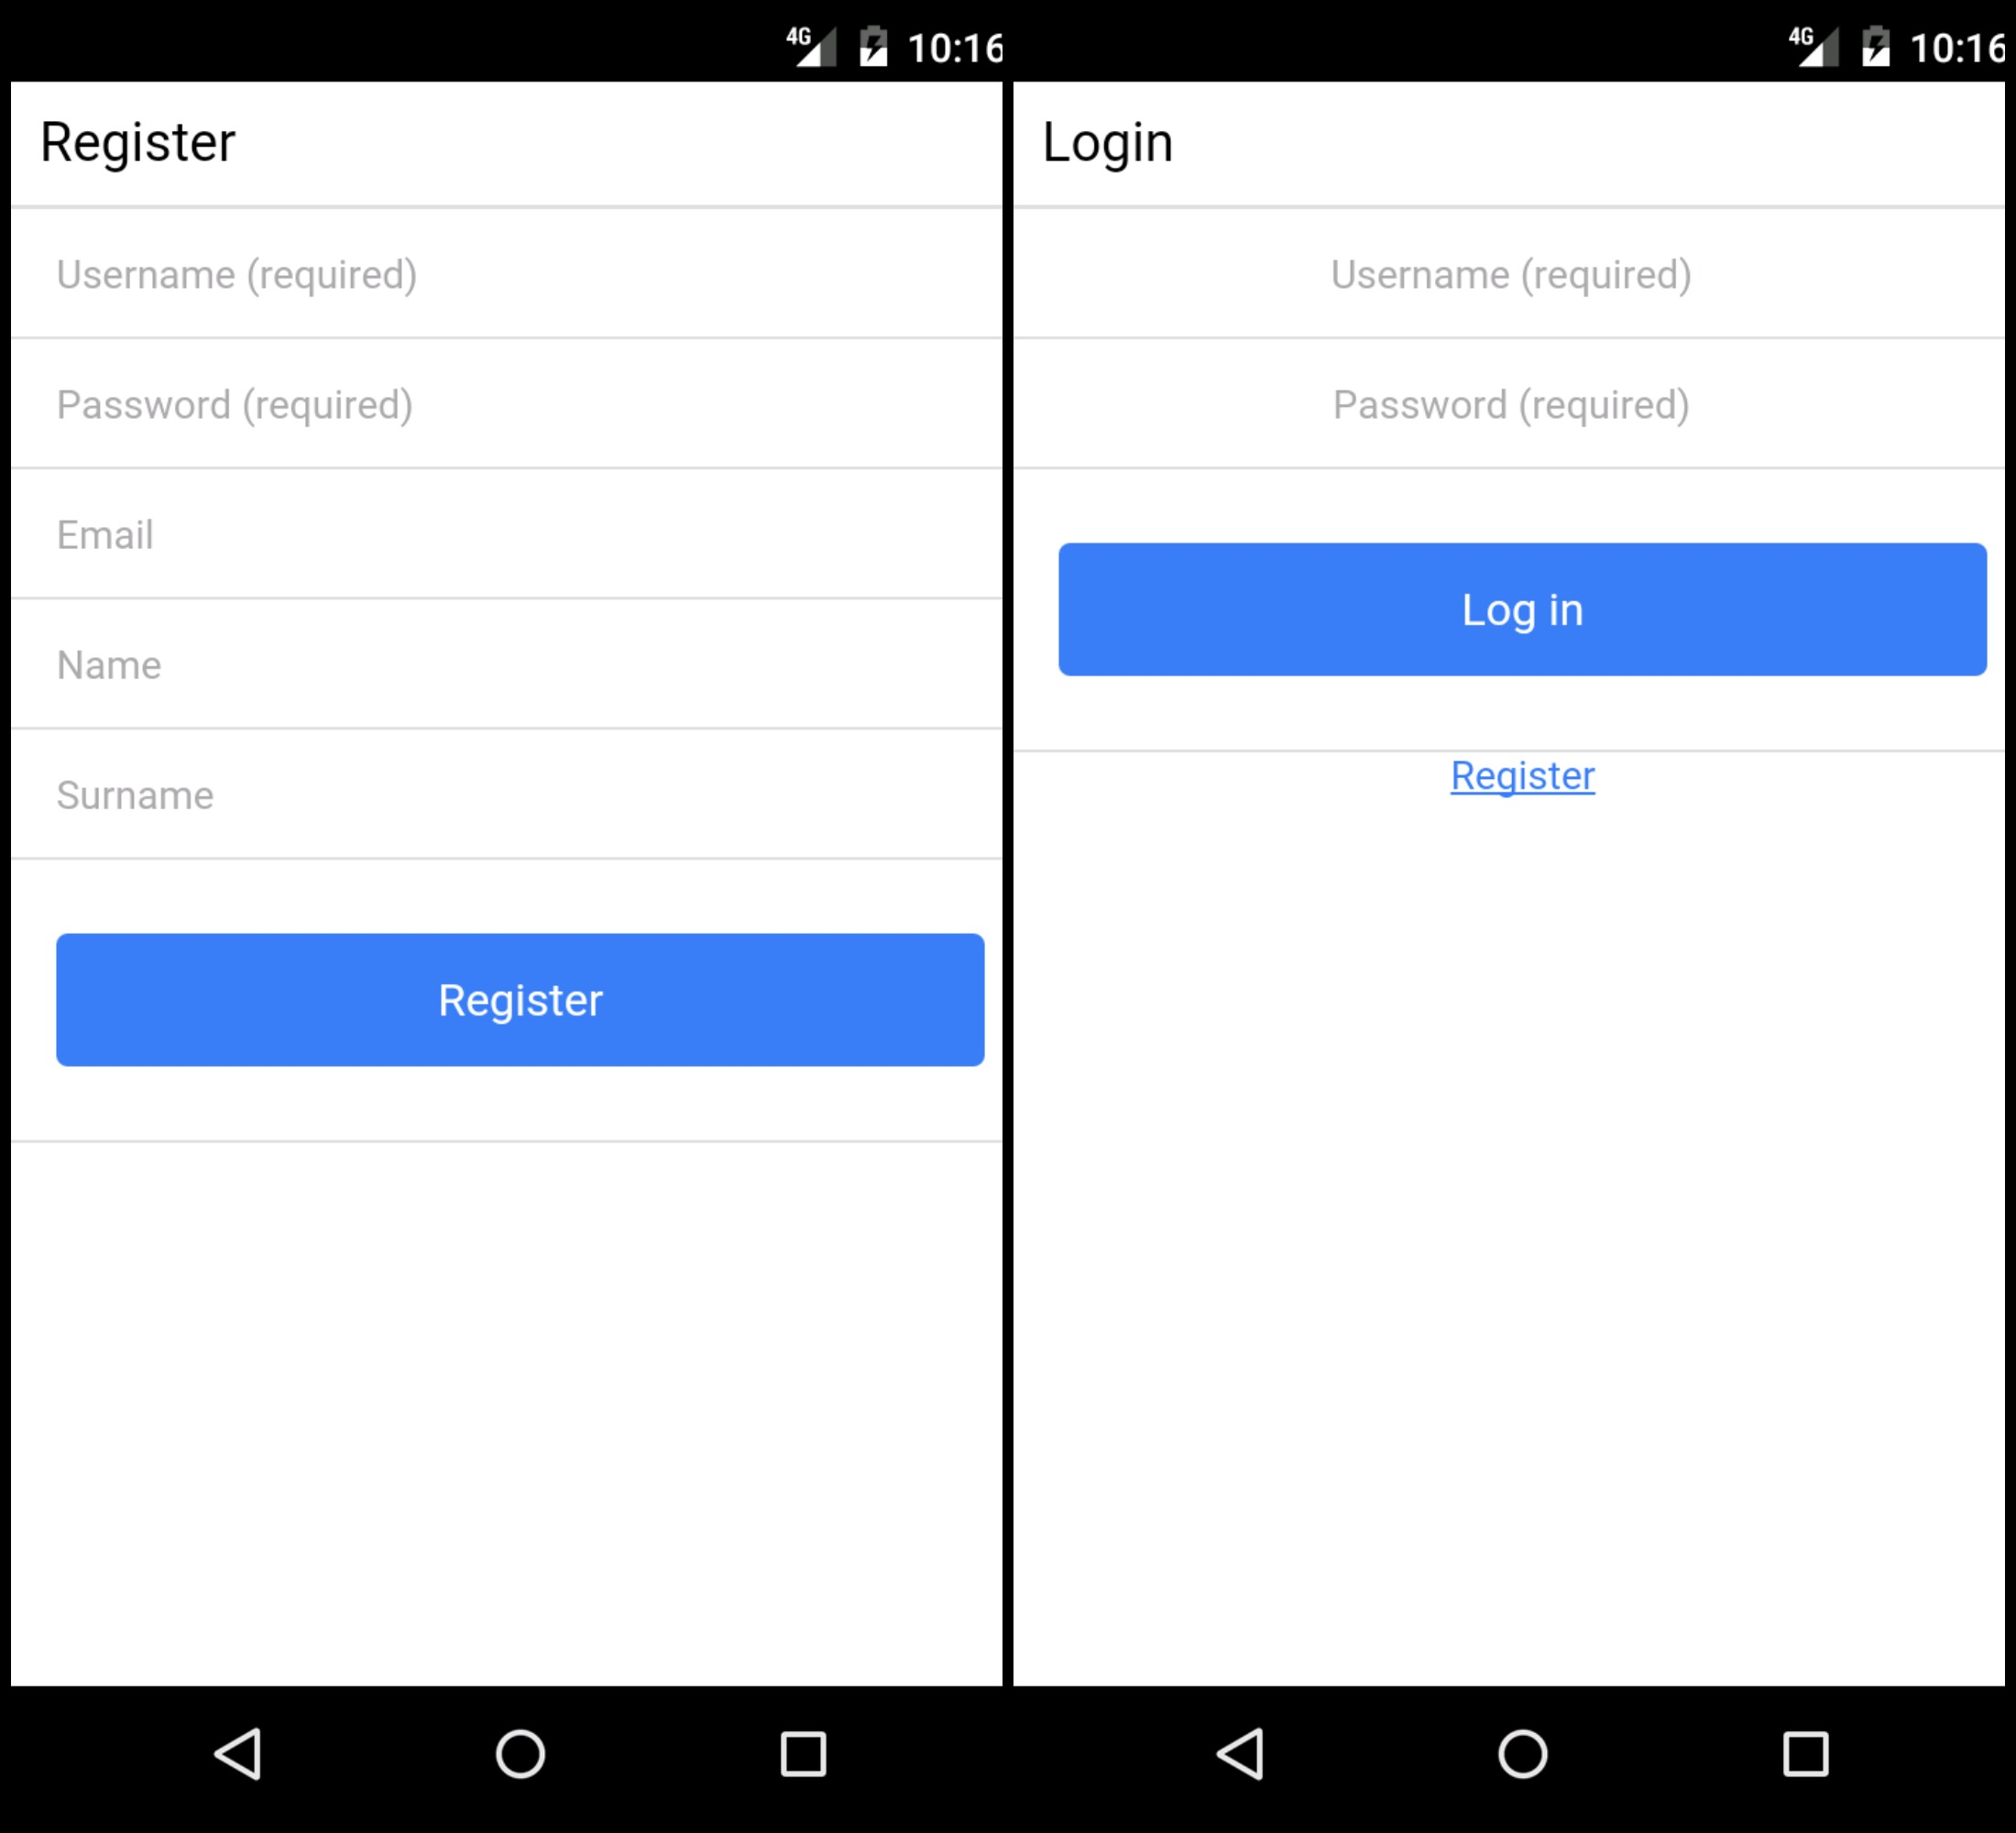
\includegraphics[width=110mm]{images/login-register.jpg}
  \caption{Εγγραφή και σύνδεση}
  \label{fig:login-register}
\end{figure}

\newpage

\subsubsection{CryptoJS}
Η βιβλιοθήκη CryptoJS προσφέρει μια μεγάλη γκάμα αλγόριθμων κρυπτογράφησης σε Javascript. Στη προκειμένη περίπτωση ο αλγόριθμος που χρησιμοποιήσαμε είναι ο AES. Όπως παρατηρούμε στον αλγόριθμο \ref{lst:encryption} πριν την ολοκλήρωση της εγγραφής του χρήστη φροντίζουμε όλα τα στοιχεία του χρήστη να αποσταλούν κρυπτογραφημένα με κλειδί τον κωδικό του. Έτσι επιτυγχάνεται η ανωνυμία του χρήστη καθώς μόνο αυτός έχει τη δυνατότητα να αποκρυπτογραφήσει και να εμφανίσει τα στοιχεία του.

\begin{lstlisting}[language=Java, caption=Κρυπτογράφηση Στοιχείων, label={lst:encryption}]

 $scope.doRegister = function () {
    $scope.encryptUserInformation();
    LoginService.register($scope.registerInfo).then(function (response) {
      $scope.closeRegister();
    });

  };

 $scope.encryptUserInformation = function () {
    $scope.registerInfo.email = $scope.encryptValue($scope.registerInfo.email);
    $scope.registerInfo.name = $scope.encryptValue($scope.registerInfo.name);
    $scope.registerInfo.surname = $scope.encryptValue($scope.registerInfo.surname);
  }

  $scope.encryptValue = function (value) {
    var text = CryptoJS.AES.encrypt(value, $scope.registerInfo.password);
    return text.toString();
  }
\end{lstlisting}

\subsection{Παρακολούθηση τοποθεσιών}
Μετά την εγγραφή και σύνδεση του, ο χρήστης βλέπει στην αρχική σελίδα, όπως παρουσιάζεται στο διάγραμμα ~\ref{fig:watch-position}, στην οποία έχει τη δυνατότητα εκκίνησης παρακολούθησης των τοποθεσιών του.

\begin{figure}[h]
  \centering
  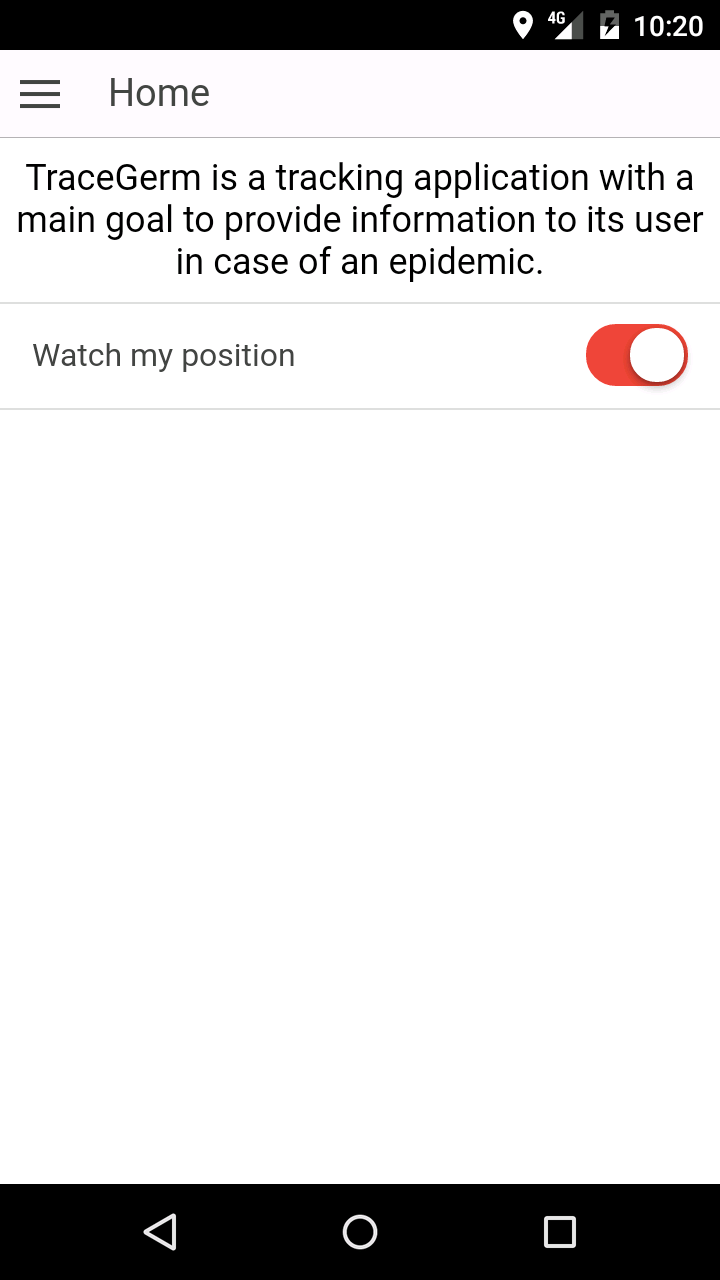
\includegraphics[width=60mm]{images/watch-position.png}
  \caption{Αρχική σελίδα εφαρμογής}
  \label{fig:watch-position}
\end{figure}

\newpage

Μετά την επιλογή του χρήστη να εκκινήσει τη παρακολούθηση, η εφαρμογή εκτελεί τον κώδικα που εμφανίζεται στον αλγόριθμο ~\ref{lst:watch-position}. Κάνοντας χρήση των δυνατοτήτων του Cordova framework λαμβάνουμε τις τοποθεσίες του χρήστη και τις αποστέλλουμε στον εξυπηρετητή για επεξεργασία και αποθήκευση.

\begin{lstlisting}[language=Java, caption=Παρακολούθηση τοποθεσιών, label={lst:watch-position}]
watchPosition: function () {
      watch = $cordovaGeolocation.watchPosition(watchOptions);
      watch.then(
        null,
        function (err) {
          console.log(JSON.stringify(err));
        },
        function (rawPosition) {
          var position = {
            position: {
              latitude: rawPosition.coords.latitude,
              longitude: rawPosition.coords.longitude
            },
            accuracy: rawPosition.coords.accuracy,
            timestamp: rawPosition.timestamp
          };
          HttpSecure.post(apiUrl + '/places', position).success(function (response) {
            console.log(JSON.stringify(response));
          }).catch(function (response) {
            console.log(JSON.stringify(response));
          });
        });
    }
\end{lstlisting}

\subsection{Συναγερμοί Χρήστη}
Πηγαίνοντας στη σελίδα των συναγερμών, ο χρήστης έχει τη δυνατότητα δημιουργίας ενός καινούριου συναγερμού, τον οποίο συναγερμό λαμβάνουν οι υπηρεσίες υγείας και αποδέχονται ή όχι. Επιπλέον δίνεται στο χρήστη η δυνατότητα εγγραφής και παραλαβής ενημερώσεων σε περίπτωση που έχει βρεθεί στην ίδια τοποθεσία με κάποιον άλλο χρήστη του οποίου ο συναγερμός έχει γίνει αποδεκτός από τις υπηρεσίες υγείας. Στο διάγραμμα ~\ref{lst:watch-position} βλέπουμε τις δύο παραπάνω δυνατότητες. 

\begin{figure}[h]
  \centering
  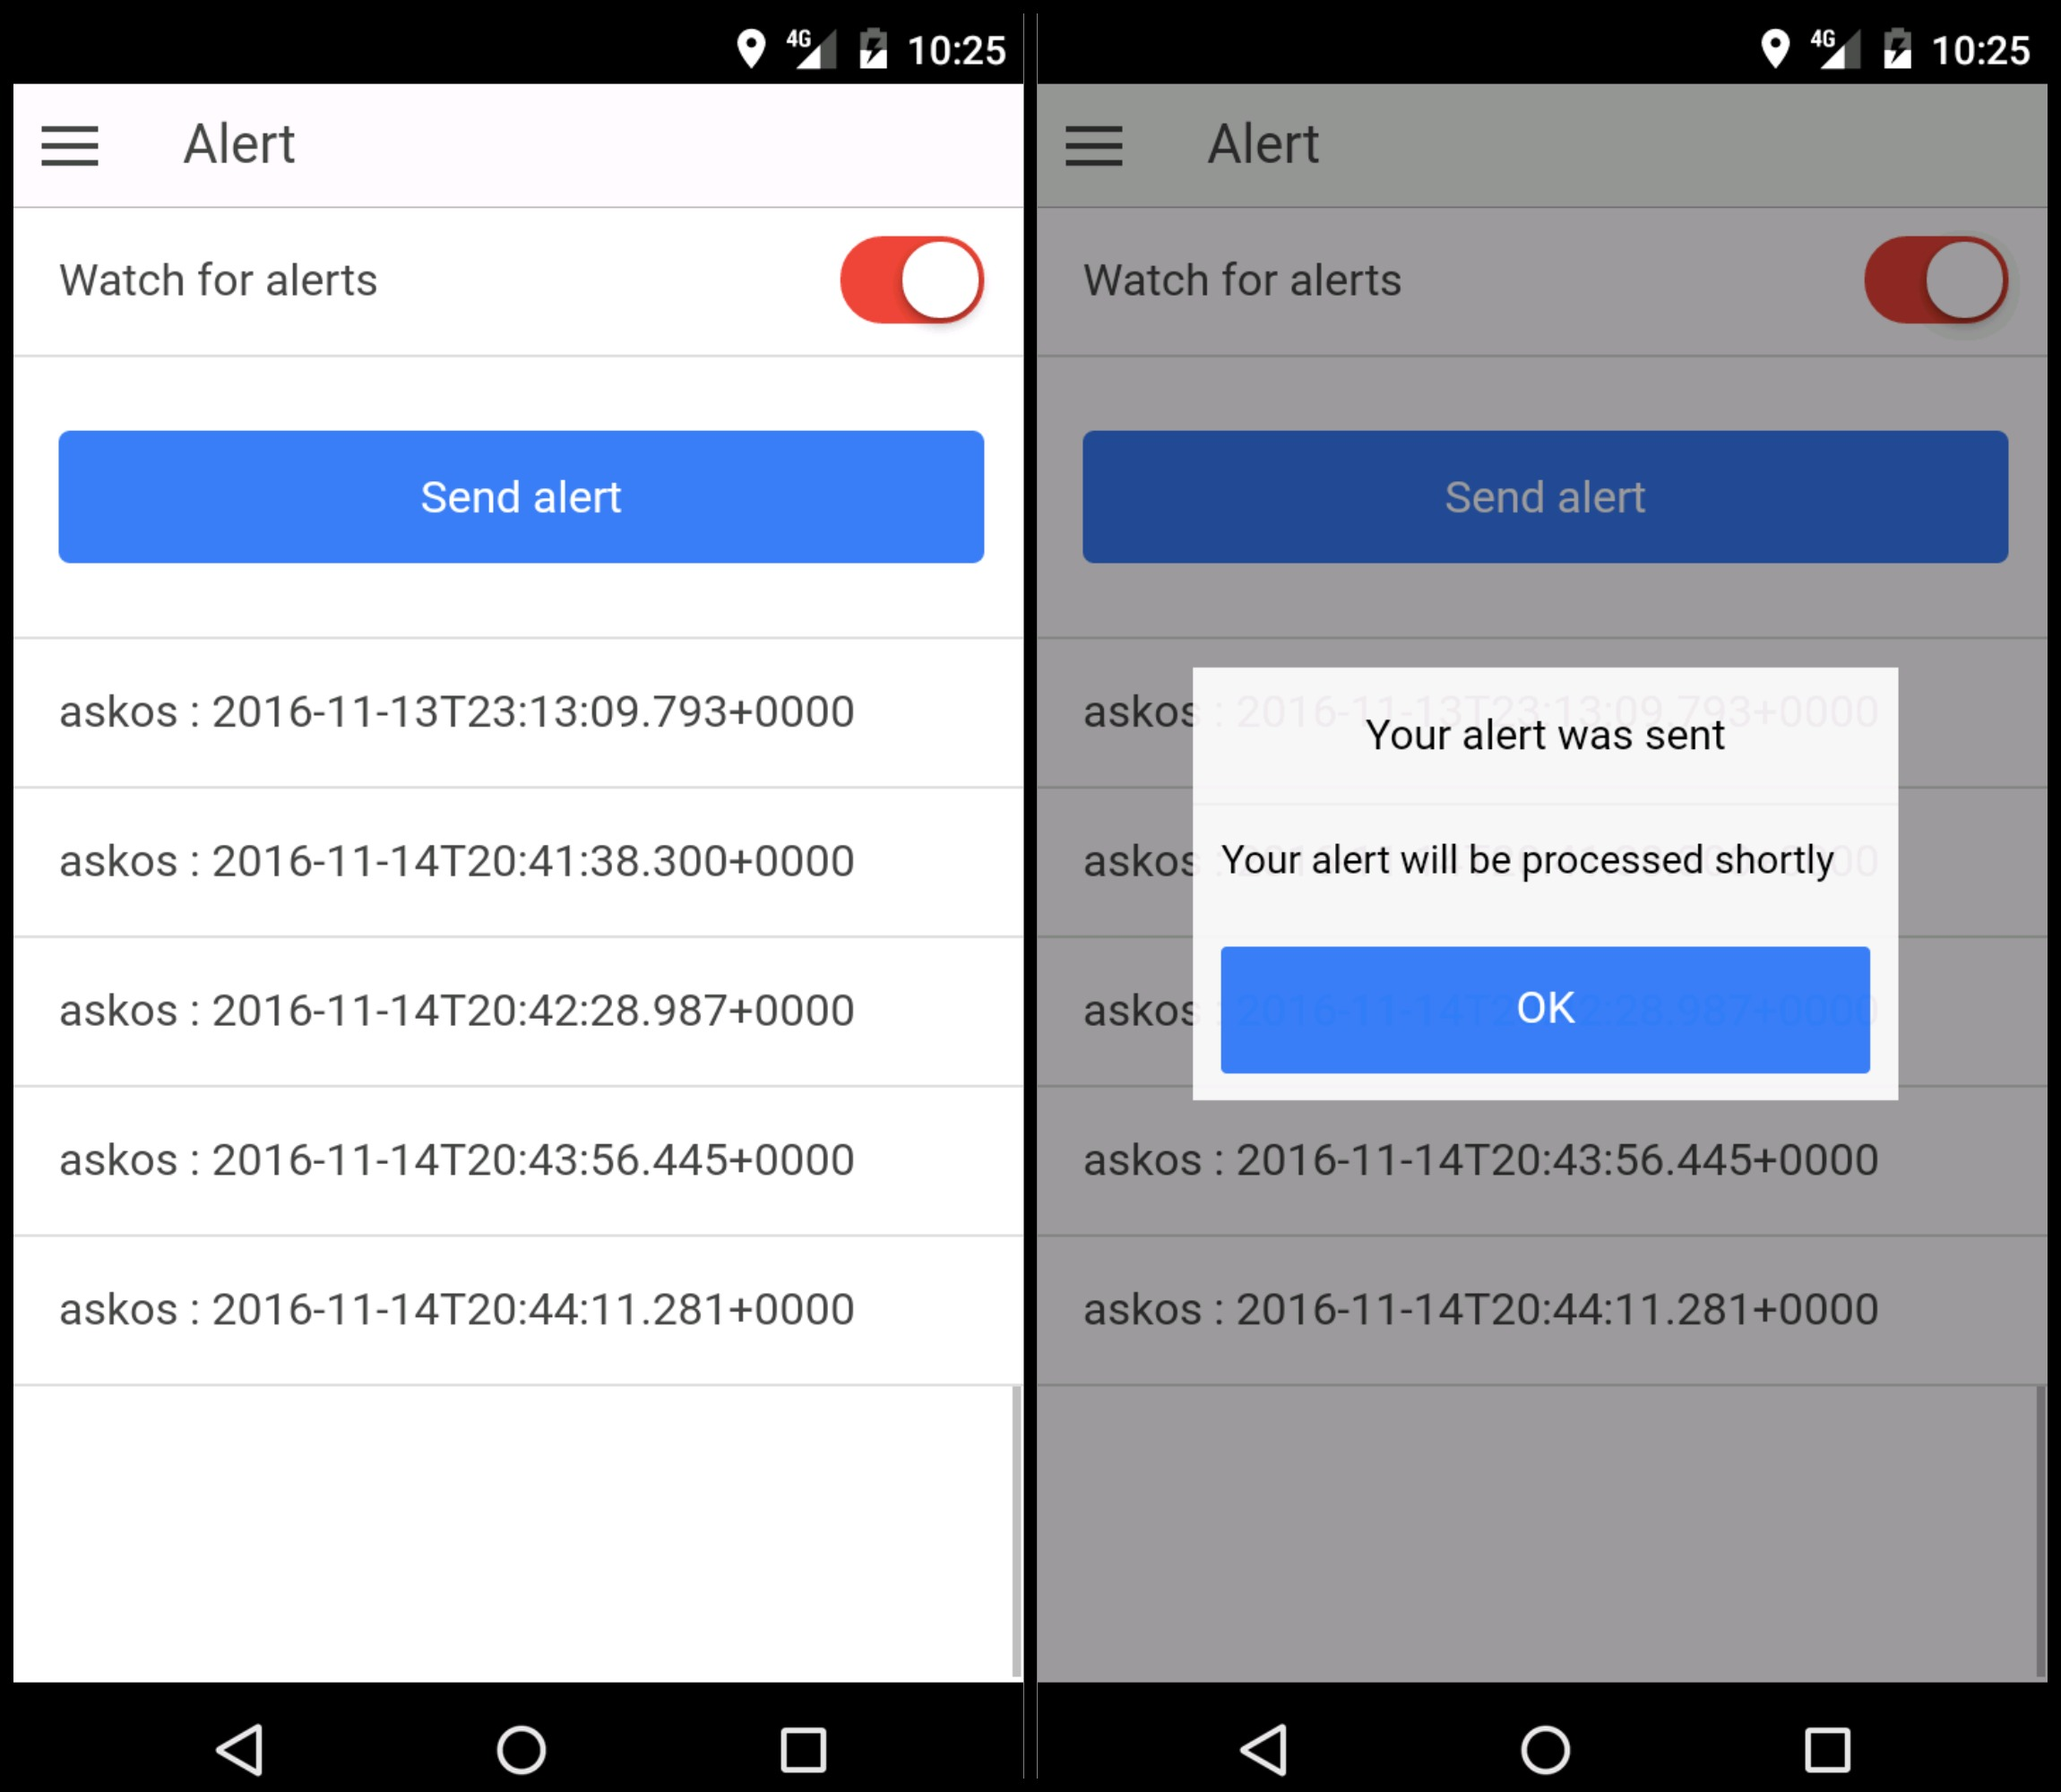
\includegraphics[width=100mm]{images/alerts.jpg}
  \caption{Συναγερμοί}
  \label{fig:alerts}
\end{figure}

\newpage

Ένα σημείο στο οποίο θα πρέπει να δώσουμε βαρύτητα είναι ο τρόπος με τον οποίο ο χρήστης παρακολουθεί για καινούριες ενημερώσεις. Κάνοντας χρήση του μοτίβου publish/subscribe (Αλγόριθμος ~\ref{fig:alerts}) ο χρήστης κάνει έγγραφή στο θέμα των ενημερώσεων οι οποίες τον απασχολούν με αποτέλεσμα να ανοίγεται ένας αγωγός επικοινωνίας με το πρωτόκολλο websocket μεταξύ της συσκευής του χρήστη και του εξυπηρετητή.

\begin{lstlisting}[language=Java, caption=Publish/Subscribe για ενημερώσεις, label={lst:publish_subscribe_notifications}]
$scope.startWatchingAlert = function () {
    $ionicPlatform.ready(function() {
      $scope.socket = new SockJS(apiUrl+'/tracegerm-websocket');
      $scope.stompClient = Stomp.over($scope.socket);
      $scope.stompClient.connect({}, function (frame) {
        $cordovaPreferences.fetch('User')
          .success(function (response) {
            $scope.stompClient.subscribe('/topic/notifications/'+ response.username, function (notification) {
              cordova.plugins.notification.local.schedule({
                title: "Alert!",
                message: "A new notification has appeared"
              });
              $scope.notifications.push(JSON.parse(notification.body));
              $scope.$apply();
            });
          })
      });
    })
  };
\end{lstlisting}

Καθώς αυτός ο αγωγός επικοινωνίας είναι συνεχώς ανοιχτός, ο χρήστης λαμβάνει άμεσα καινούριες ενημερώσεις. Σε αυτό το σημείο είναι σημαντικό να αναφέρουμε ότι για να αποφύγουμε τυχόν χαμένες ειδοποιήσεις οι οποίες δημιουργήθηκαν όταν ο χρήστης για κάποιο λόγο δεν ήταν συνδεδεμένος, φροντίζουμε να φορτώσουμε όλες τις ειδοποιήσεις τις οποίες ο χρήστης δεν έχει αποδεχτεί ακόμη, οι οποίες εμφανίζονται σε μορφή λίστας. Στο διάγραμμα ~\ref{fig:notifications} μπορούμε να παρατηρήσουμε και τις δύο παραπάνω καταστάσεις.   

\begin{figure}[h]
  \centering
  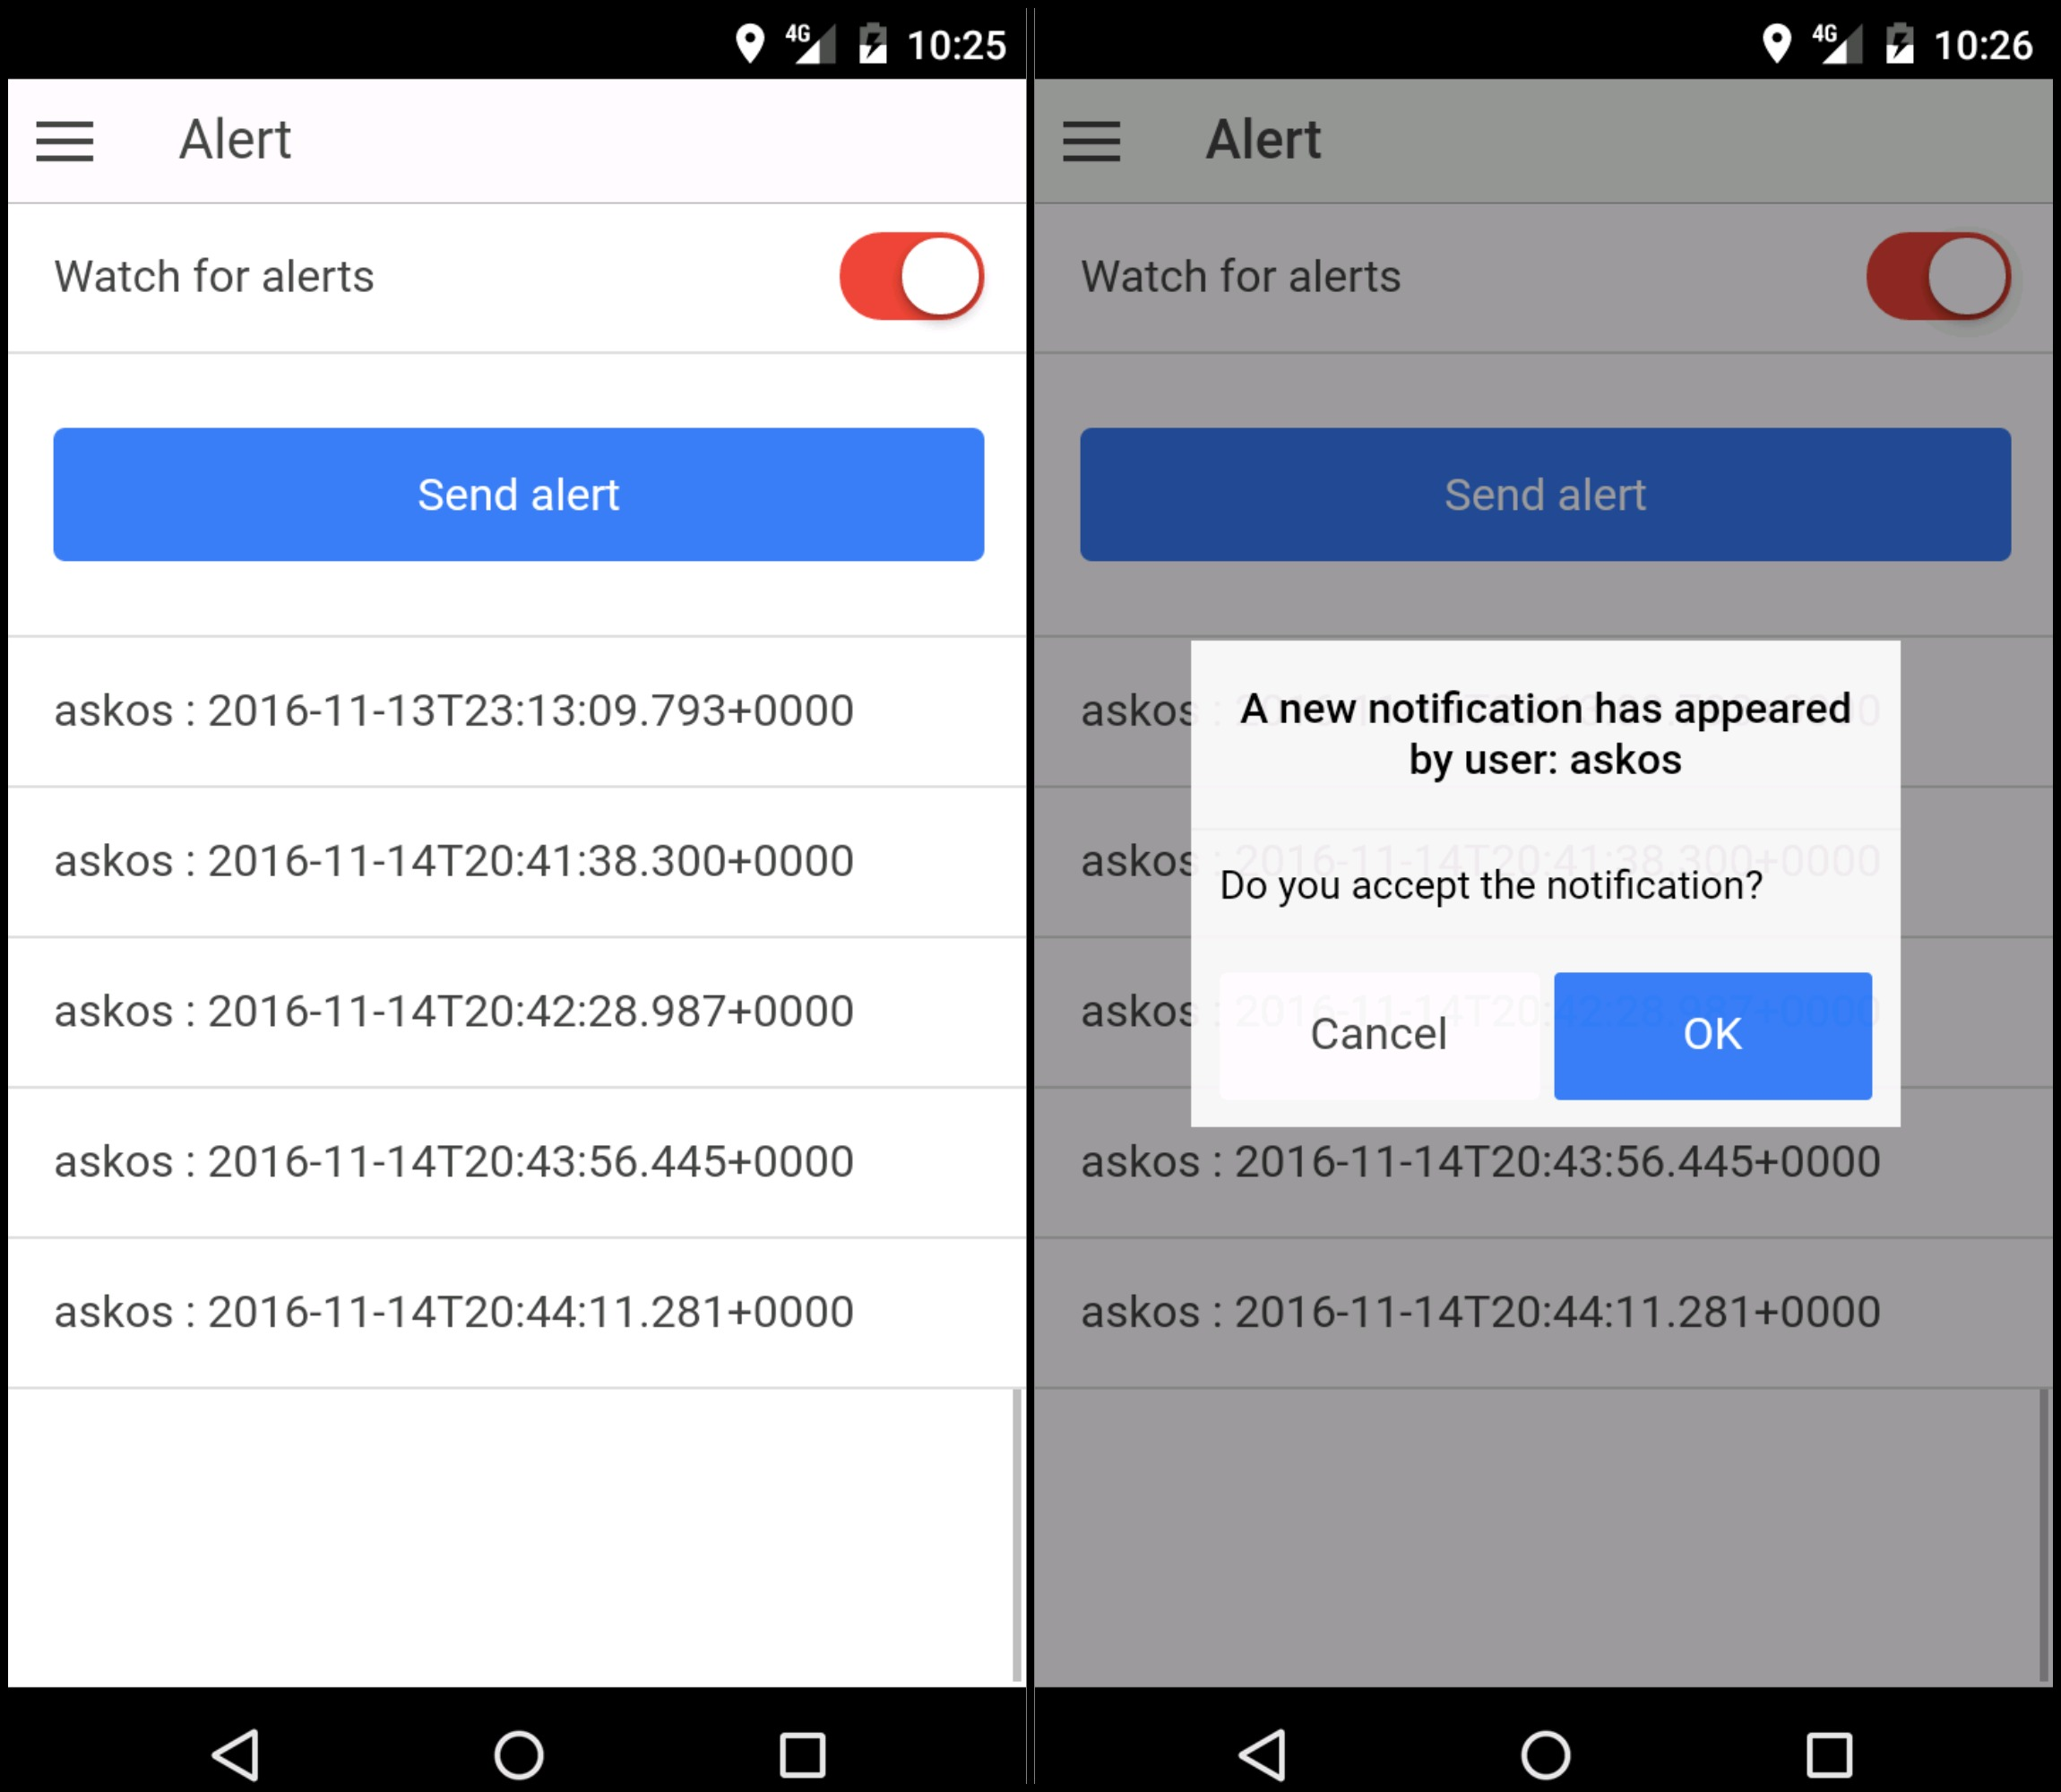
\includegraphics[width=100mm]{images/notifications.jpg}
  \caption{Ενημερώσεις}
  \label{fig:notifications}
\end{figure}

\newpage
\subsection{Τοποθεσίες Χρήστη}
Τέλος, ο χρήστης έχει τη δυνατότητα να δει τις τελευταίες τοποθεσίες τις οποίες επισκέφθηκε μέσω της σελίδας προφίλ. Για να γίνει η εμφάνιση των τοποθεσιών αυτών με ένα φιλικό τρόπο απέναντι στο χρήστης, αποφασίστηκε να γίνει χρήση της υπηρεσίας Google Maps. Έτσι ο χρήστης έχει τη δυνατότητα να δει τις τοποθεσίες του άμεσα σε ένα χάρτη (διάγραμμα ~\ref{fig:locations})  αντί μιας λίστας με γεωγραφικά πλάτη και μήκη.

\begin{figure}[h]
  \centering
  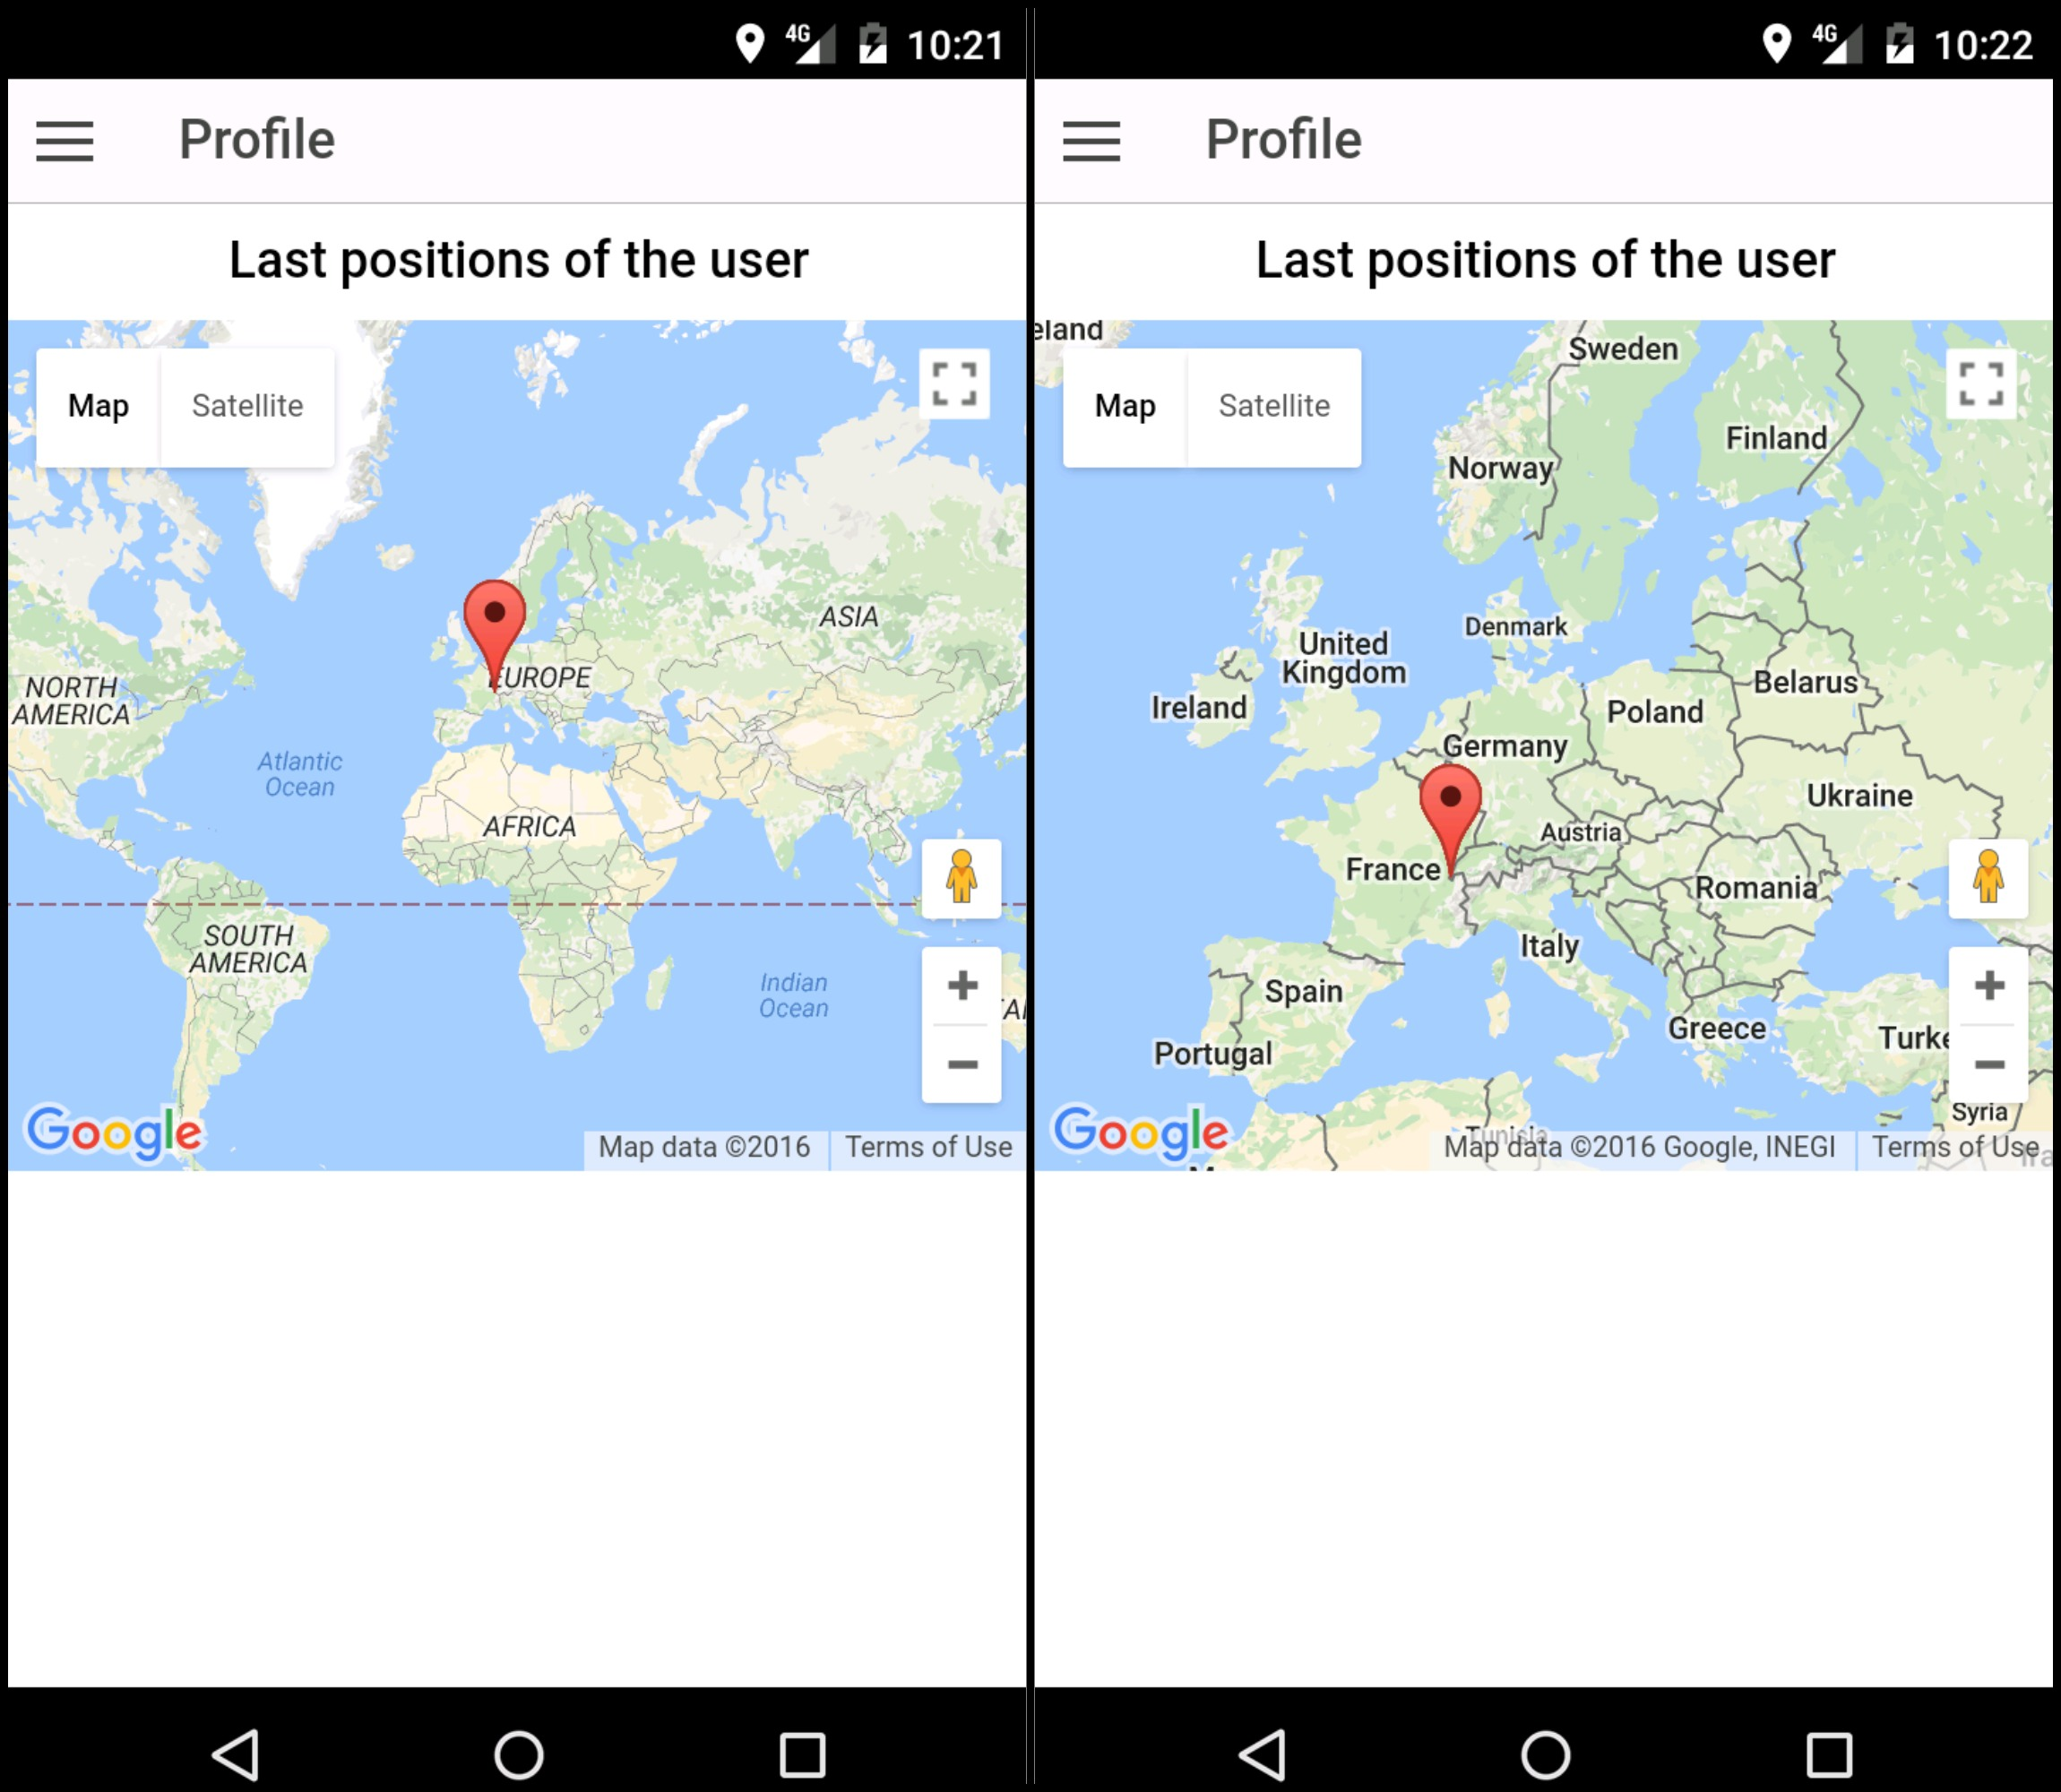
\includegraphics[width=100mm]{images/profile.jpg}
  \caption{Τοποθεσίες χρήστη}
  \label{fig:locations}
\end{figure}

\section{Ροή της Διαδικτυακής Εφαρμογής}
Η διαδικτυακή εφαρμογή είναι σαφώς πιο απλή από την εφαρμογή κινητών συσκευών. Παρακάτω θα παρουσιάσουμε την διεπαφή χρήστη καθώς και τις λειτουργίες της.

\subsection{Είσοδος Υπαλλήλου Υπηρεσιών Υγείας}
Στην αρχική σελίδα της διαδικτυακής εφαρμογής ζητάμε από τους υπαλλήλους των υπηρεσιών υγείας να εισέλθουν κάνοντας χρήση ενός λογαριασμού ο οποίος έχει τον ρόλο διαχειριστή. Με αυτό το τρόπο φροντίζουμε οι χρήστες μας να είναι εξουσιοδοτημένοι και τα στοιχεία των χρηστών μας ασφαλή. Καθώς οι απαραίτητοι έλεγχοι γίνονται στο επίπεδο του εξυπηρετητή, θα αποφύγουμε να μπούμε σε λεπτομέρειες σε αυτό το σημείο και θα αναφερθούμε περαιτέρω αργότερα.

\begin{figure}[h]
  \centering
  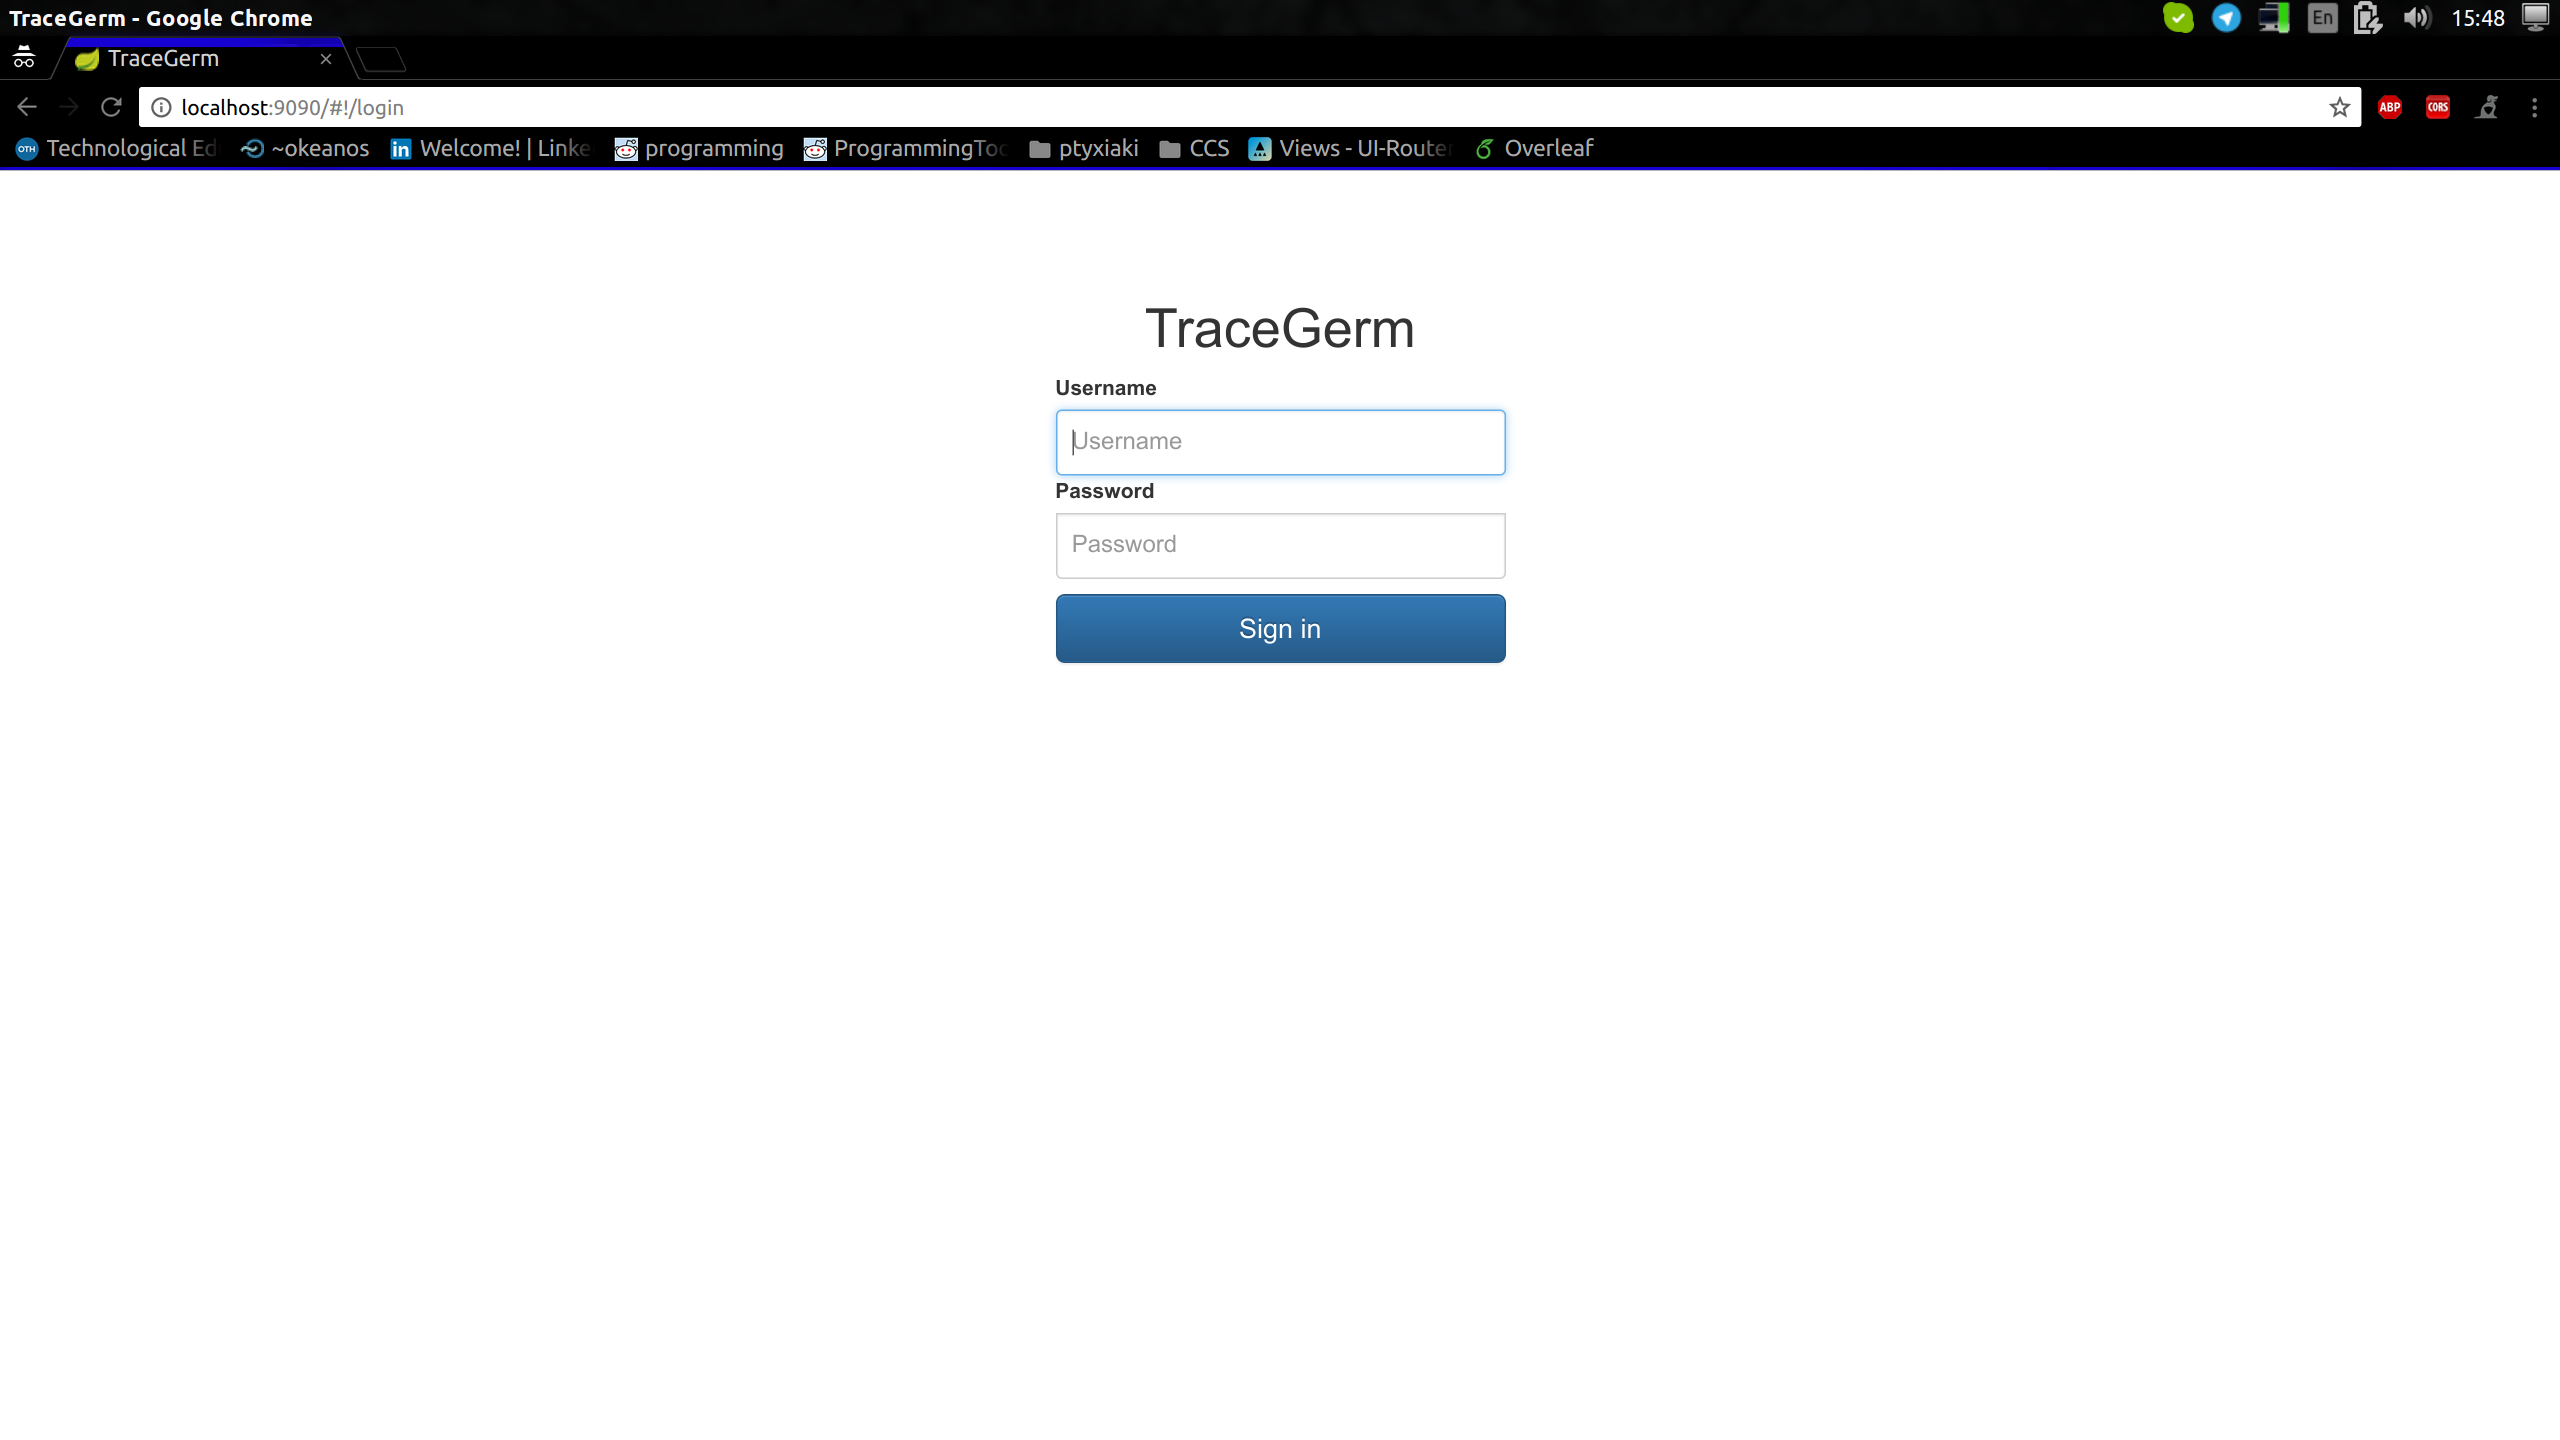
\includegraphics[width=150mm]{images/login.png}
  \caption{Είσοδος Υπαλλήλου Υπηρεσιών Υγείας}
  \label{fig:login-webapp}
\end{figure}

\subsection{Σελίδα συναγερμών}
Καθώς οι υπάλληλοι έχουν εισέλθει στη σελίδα συναγερμών, έχουν τη δυνατότητα να λαμβάνουν σε πραγματικό χρόνο νέους συναγερμούς από τους χρήστες με το πρότυπο publish/subscribe. Κατά συνέπεια οι υπάλληλοι μπορούν να αποδεχτούν ή όχι έναν συναγερμό. Λόγω της κρισιμότητας μιας τέτοιας απόφασης αποφασίστηκε να δοθεί ο πλήρης έλεγχος στους ανθρώπους χωρίς επέμβαση κάποιου αλγόριθμου. Έτσι εάν ένας υπάλληλος αποφασίσει ότι πρέπει να αποδεχτεί τον συναγερμό ενός χρήστη τότε φροντίζουμε να καλέσουμε τον απαραίτητο αλγόριθμο στον εξυπηρετητή για να ενημερώσουμε όλους τους χρήστες οι οποίοι μπορεί να ήρθαν σε επαφή μαζί του.

\begin{figure}[h]
  \centering
  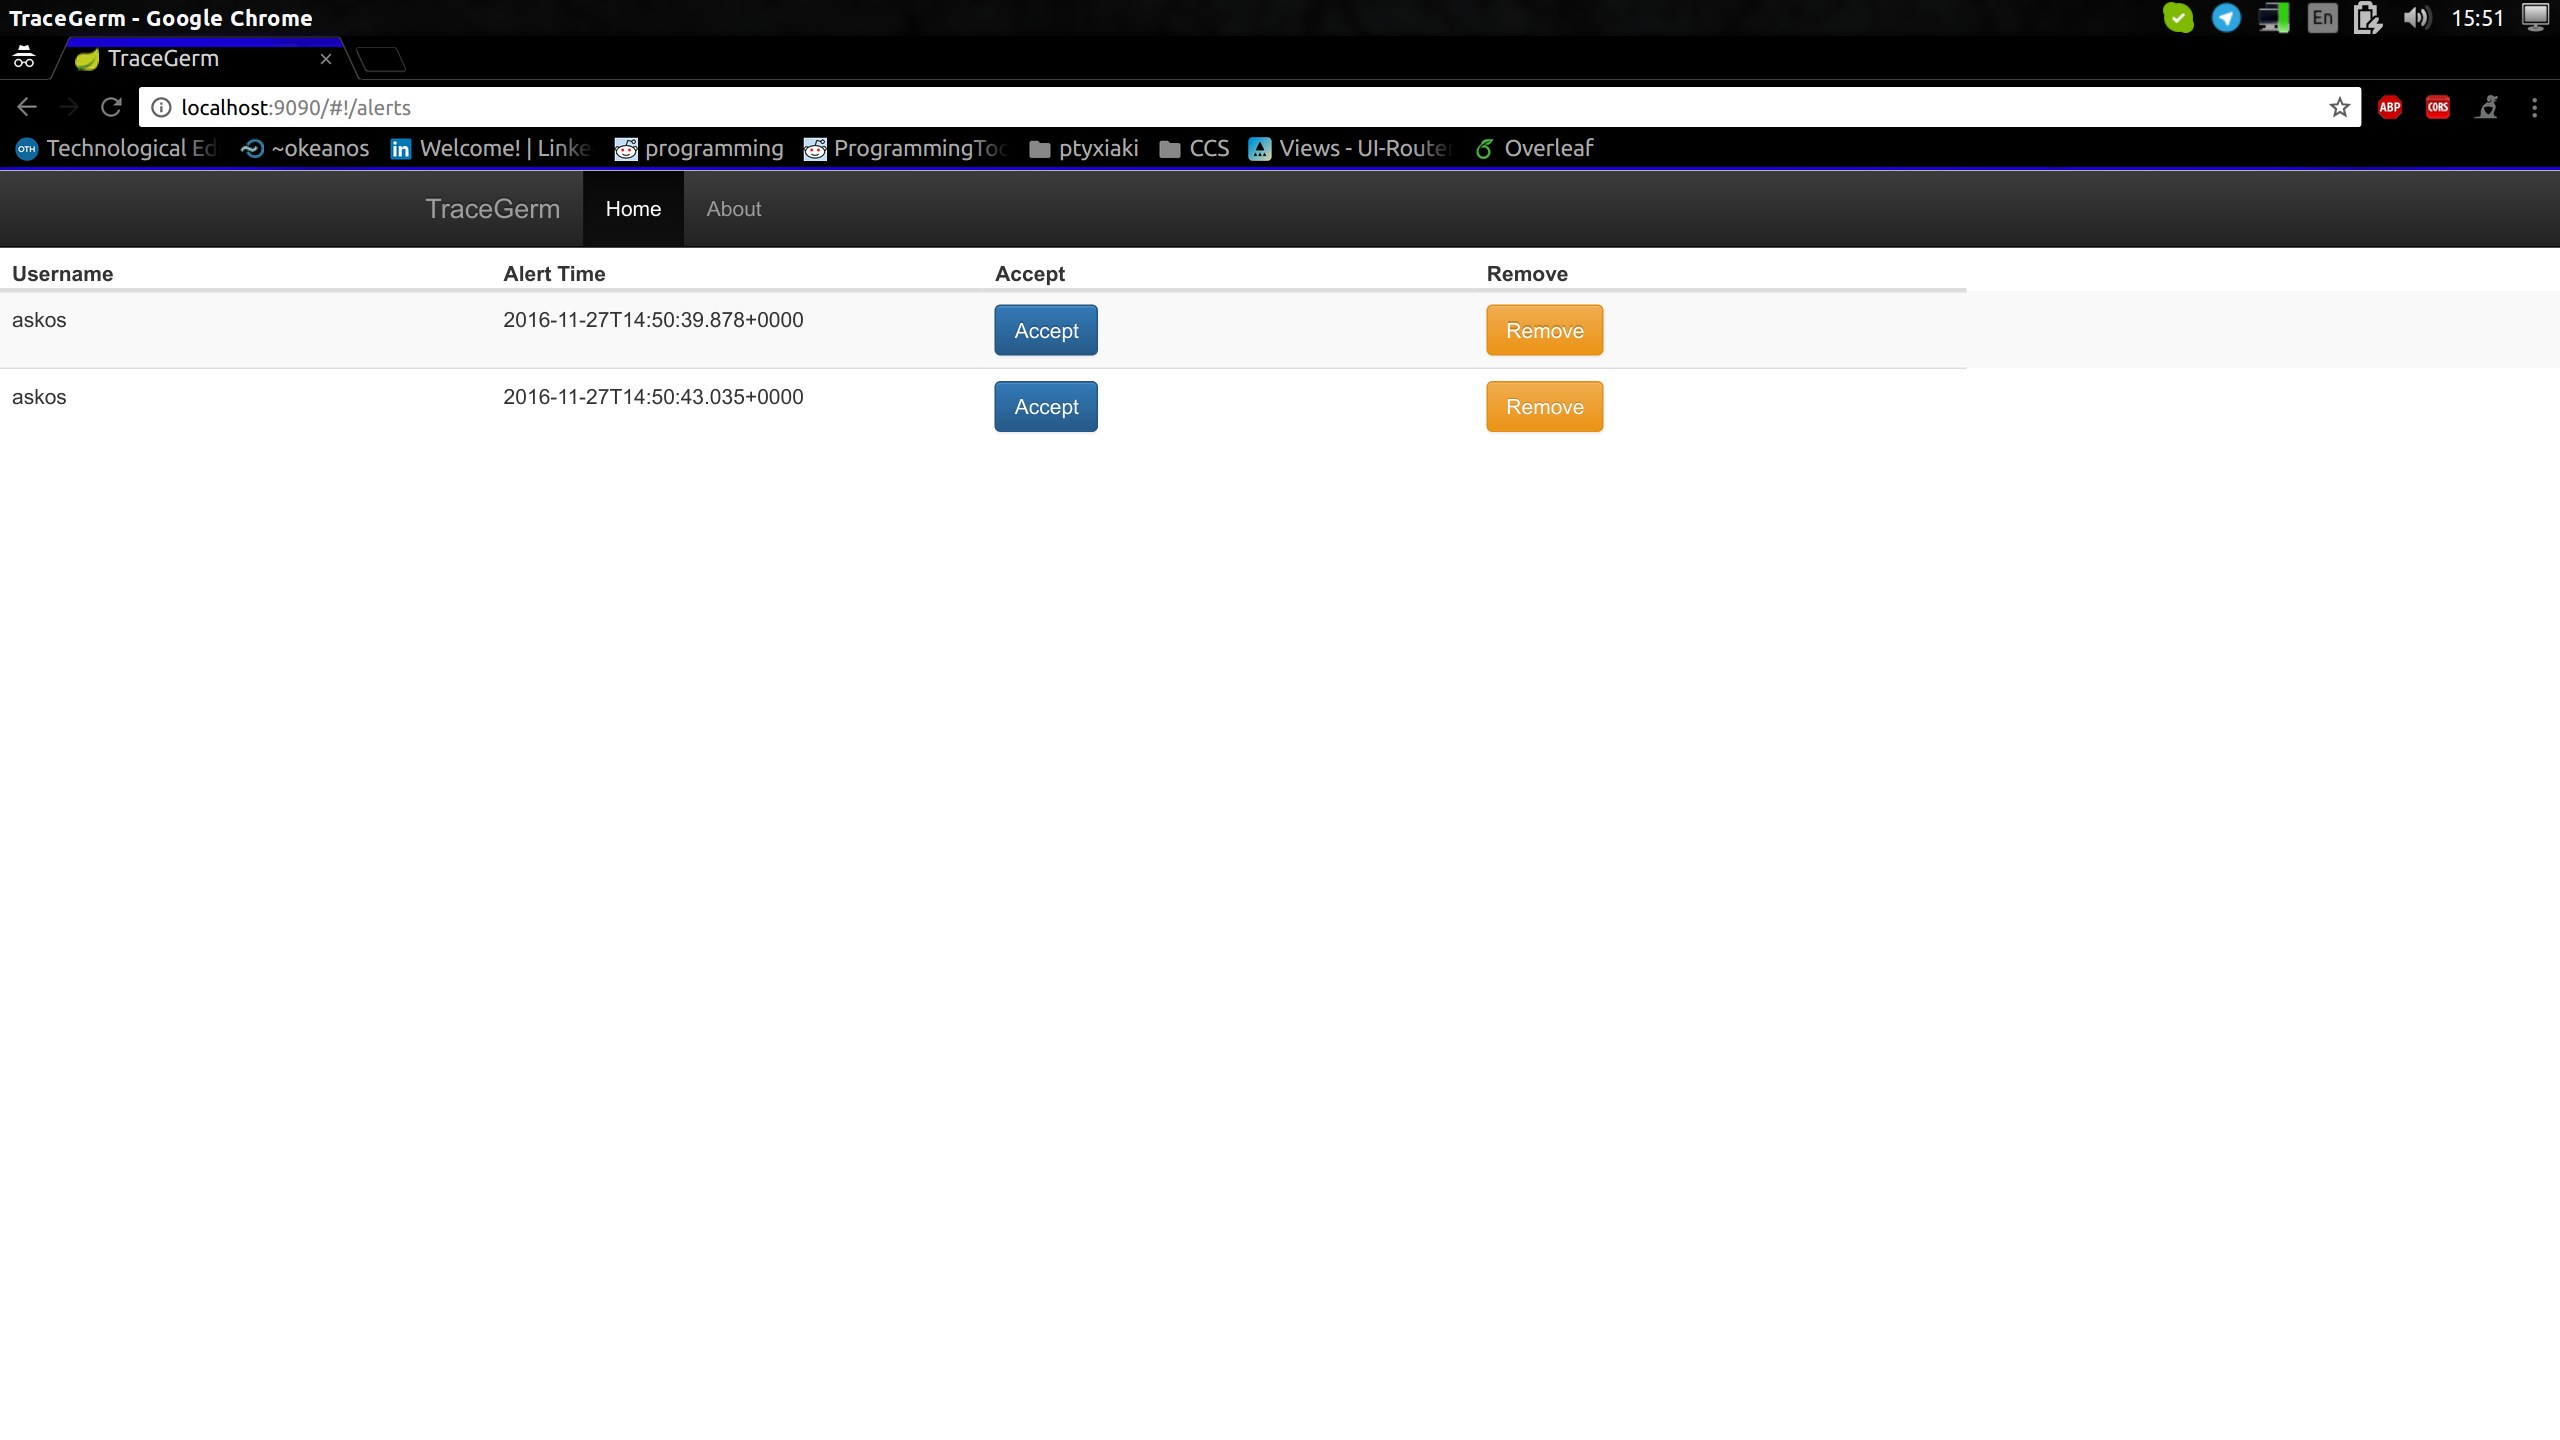
\includegraphics[width=150mm]{images/alerts.png}
  \caption{Εμφάνιση συναγερμών}
  \label{fig:login-webapp}
\end{figure}

\newpage

\section{Web Service}
Παρακάτω θα παρουσιάσουμε λεπτομερώς τα πιο καίρια κομμάτια του εξυπηρετητή. Θα παρουσιάσουμε το μοντέλο της εφαρμογής μας καθώς και τα πιο σημαντικά κομμάτια όπως ο αλγόριθμος αποστολής ειδοποιήσεων στους χρήστες καθώς και οι διαφορετικοί τρόποι επικοινωνίας.

\subsection{Μοντέλο Εφαρμογής}
Το μοντέλο της εφαρμογής αποτελείται από τα αντικείμενα τα οποία κάνουμε χρήση κατά τη διάρκεια εκτέλεσης του συστήματος για να επεξεργαστούμε, εμφανίσουμε και φυσικά να δημιουργήσουμε τα δεδομένα του συστήματος μας. Συγκεκριμένα το μοντέλο της εφαρμογής μας αποτελείτε από τέσσερις βασικές οντότητες. Στο διάγραμμα ~\ref{fig:domain-diagram} μπορούμε να δούμε το βασικό μοντέλο της εφαρμογής.

\begin{figure}[h]
  \centering
  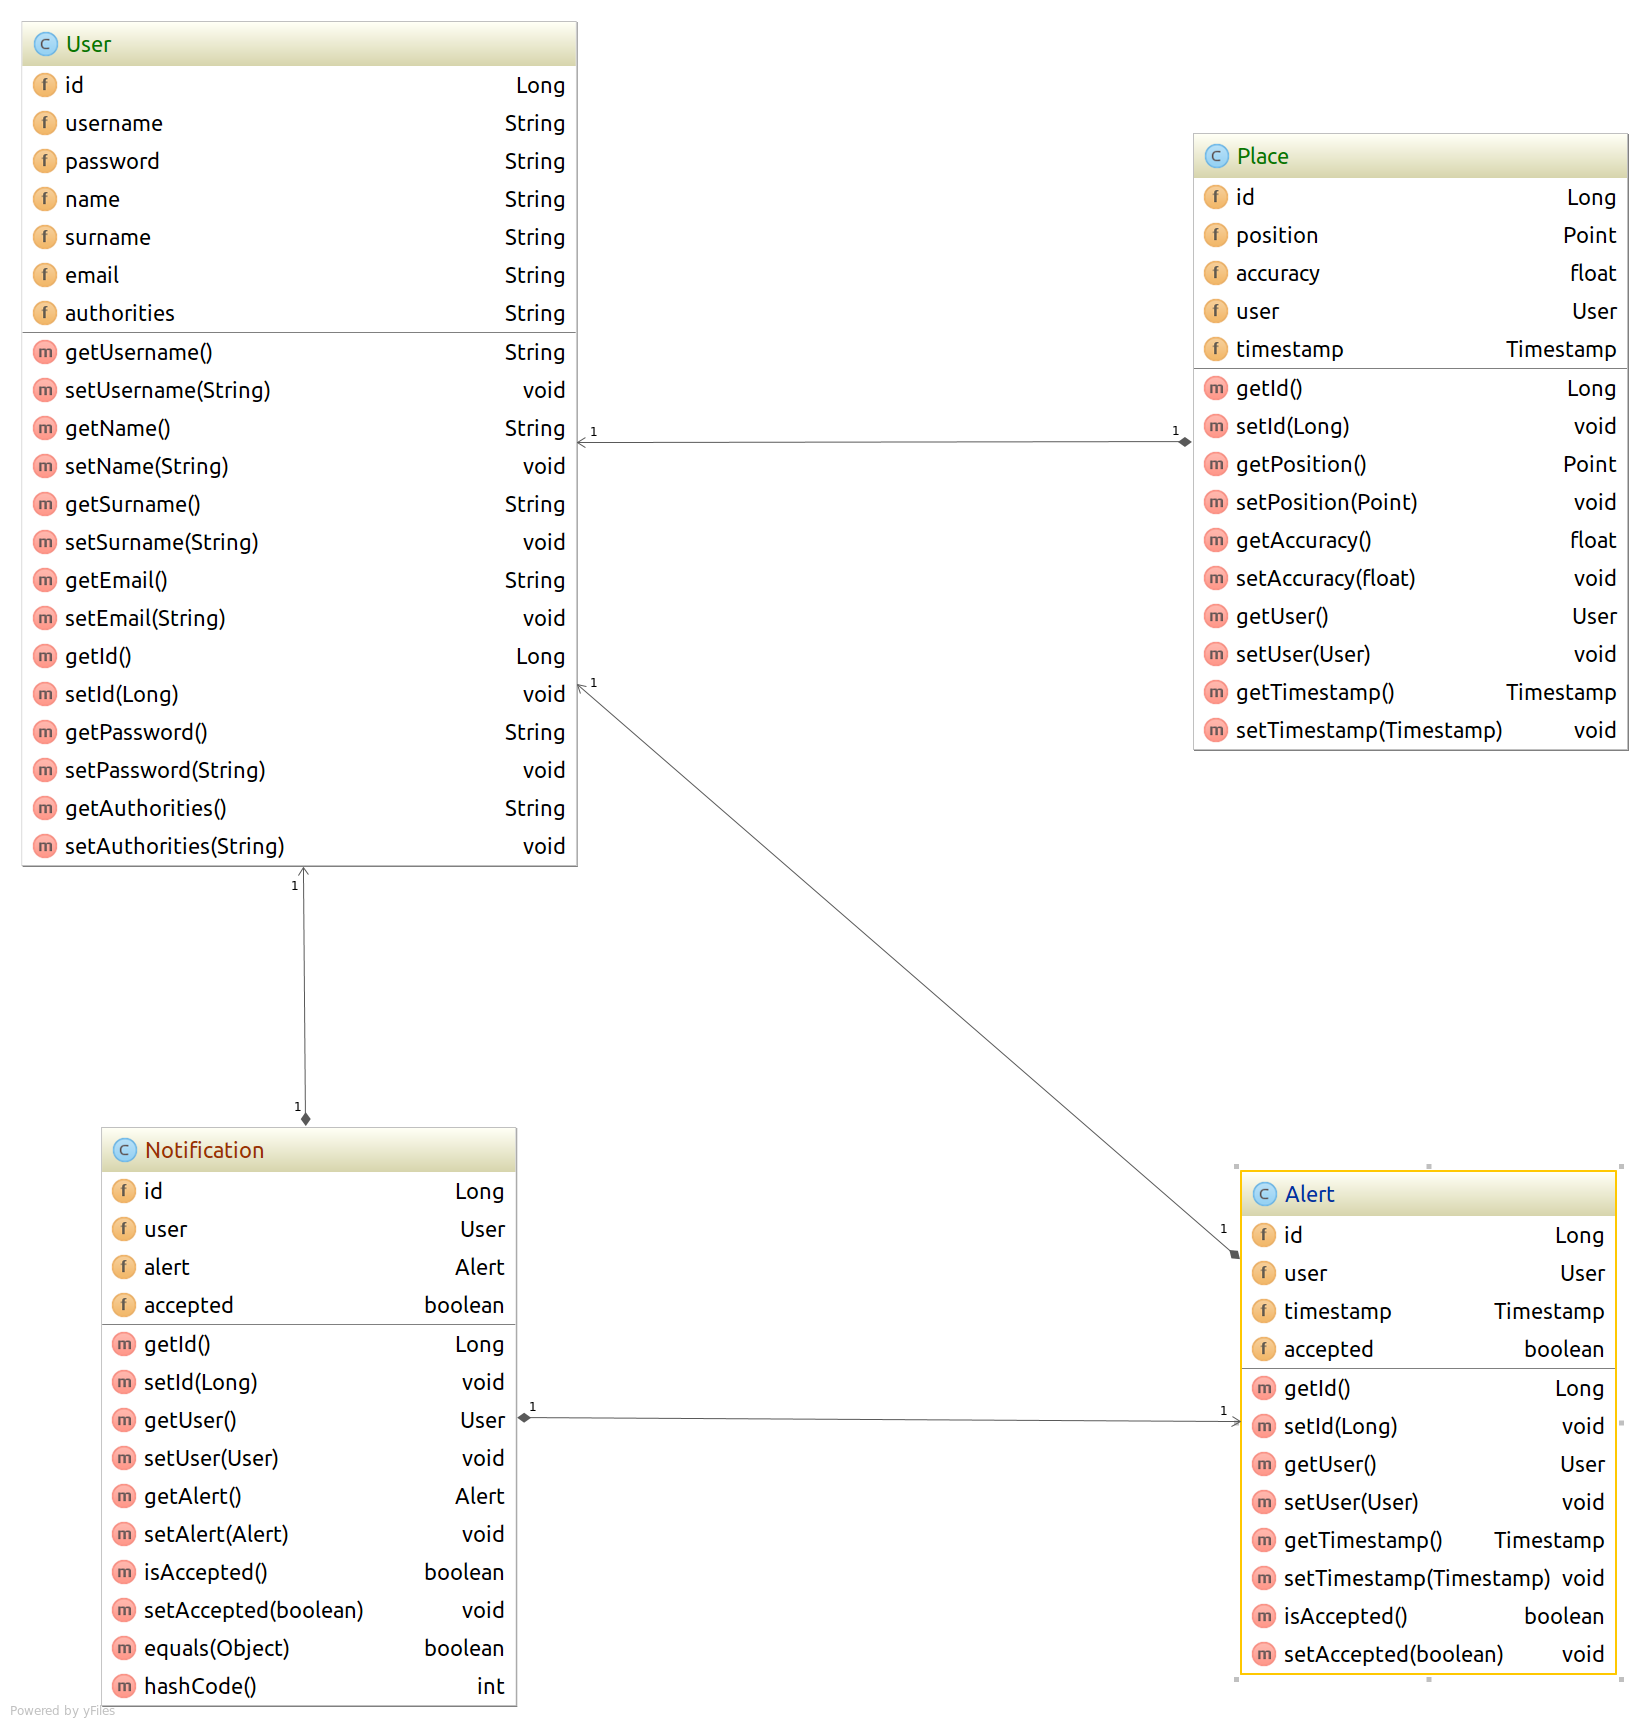
\includegraphics[width=150mm]{images/domain-diagram.png}
  \caption{Μοντέλο εφαρμογής}
  \label{fig:domain-diagram}
\end{figure}

\newpage

\subsection{Επικοινωνία με το API}
Όπως έχουμε προαναφέρει η επικοινωνία των πελατών με τον εξυπηρετητή γίνεται κατά βάση με τη χρήση του ReST API όπως επίσης και με το μοτίβο Publish/Subscribe μέσω του πρωτοκόλλου websockets. Παρακάτω θα παρουσιάσουμε εις βάθος τους δύο παραπάνω τρόπους επικοινωνίας και τις περιπτώσεις χρήσης τους καθώς και τα JSON μηνύματα τα οποία ανταλλάσσονται κατά τη διάρκεια της επικοινωνίας.

\subsection{Rest API}
Ο βασικός τρόπος επικοινωνίας γίνεται μέσω του Rest API. Οι εφαρμογές μας στέλνουν συγκεκριμένα http αιτήματα τα οποία αφού ο εξυπηρετητής μας επεξεργαστεί επιστρέφει την απαραίτητη απάντηση στον πελάτη σε μορφή JSON. Για να γίνει ξεκάθαρη η σύνταξη για την επικοινωνία, παρακάτω θα εμφανίσουμε ένα πραγματικό παράδειγμα από την εφαρμογή μας. 

\subsubsection{Αίτημα πελάτη}
Ο πελάτης δημιουργεί ένα αίτημα για την εύρεση των τελευταίων τοποθεσιών στις οποίες βρέθηκε. Το αίτημα εμφανίζεται στο κώδικα ~\ref{lst:places-request} και παρατηρούμε ότι η εφαρμογή κάνει ένα αίτημα GET αίτημα στο URI: /places/user/lastPlaces.  

\begin{lstlisting}[language=Java, caption=Αίτημα τελευταίων τοποθεσιών του χρήστη, label={lst:places-request}]
getLast10Positions: function () {
      return HttpSecure.get(apiUrl + '/places/user/lastPlaces');
    }
\end{lstlisting}

\subsubsection{Επεξεργασία εξυπηρετητή}
Ο εξυπηρετητής λαμβάνει το αίτημα στο επίπεδο των διαχειριστών όπως φαίνεται στον αλγόριθμο ~\ref{lst:places-controller}. Όταν ο υπεύθυνος διαχειριστής απολάβει το αίτημα φροντίζει να μεταφέρει το αίτημα στο επόμενο επίπεδο, το επίπεδο των υπηρεσιών.

\begin{lstlisting}[language=Java, caption=Διαχειριστής εξυπηρετητή, label={lst:places-controller}]
    
@RepositoryRestController
@RequestMapping("/api/places")
public class PlaceController {

  private final Logger logger = Logger.getLogger(this.getClass());

  @Autowired
  private UserRepository userRepository;

  private final PlaceService placeService;

  private final SecurityContextProvider securityContextProvider;

  @Autowired
  public PlaceController(PlaceService placeService, SecurityContextProvider securityContextProvider) {
    this.placeService = placeService;
    this.securityContextProvider = securityContextProvider;
  }

  @RequestMapping(value = "/user/lastPlaces", method = RequestMethod.GET)
  public ResponseEntity<?> getLast10PlacesByToken() throws AuthenticationException {
    
    User user = this.userRepository
    .findByUsername(securityContextProvider
    .getUserDetails().getUsername());
    
    return ResponseEntity
    .ok(placeService.getLast10Places(user));
  }
}

\end{lstlisting}

Το επίπεδο των υπηρεσιών είναι υπεύθυνο για την οποιαδήποτε επεξεργασία των δεδομένων πριν την αποστολή στο χρήστη. Το επίπεδο υπηρεσιών λαμβάνει τα δεδομένα από το επίπεδο δεδομένων και γίνεται εφαρμογή της λογικής του συστήματός μας όπου αυτό είναι αναγκαίο (Αλγόριθμος ~\ref{lst:places-service}).

\begin{lstlisting}[language=Java, caption=Επίπεδο υπηρεσιών εξυπηρετητή, label={lst:places-service}]
    
@Service
@Transactional
public class PlaceServiceImpl implements PlaceService {

    private final PlaceRepository placeRepository;

    @Autowired
    public PlaceServiceImpl(PlaceRepository placeRepository) {
        this.placeRepository = placeRepository;
    }

    @Override
    public List<Place> getLast10Places(User user) {
        return placeRepository.getLast10PlacesByUserId(user.getId());
    }
}

\end{lstlisting}

Τέλος το επίπεδο δεδομένων φροντίζει για την ανάκτηση των δεδομένων τα οποία ζητήθηκαν από το επίπεδο των υπηρεσιών. Στον αλγόριθμο ~\ref{lst:places-repository} μπορούμε να δούμε το ακριβές ερώτημα που εκτελείται στη βάση δεδομένων.

\begin{lstlisting}[language=Java, caption=Επίπεδο δεδομένων εξυπηρετητή, label={lst:places-repository}]
    
@RepositoryRestResource(collectionResourceRel = "places", path = "places")
public interface PlaceRepository extends JpaRepository<Place, Long> {

    @RestResource(exported = false)
    @Query(value = "select * from places where fk_user = :userId order by  timestamp desc limit 10", nativeQuery = true)
    List<Place> getLast10PlacesByUserId(@Param("userId") Long userId);
    
    

}


\end{lstlisting}

\subsubsection{Δεδομένα επιστροφής}
Έχοντας ολοκληρώσει την επεξεργασία των δεδομένων, αυτά επιστρέφονται στο πελάτη με τη μορφή JSON. Εδώ να αναφέρουμε ότι η αναπαράσταση με τη μορφή JSON δεν είναι η μοναδική που μπορεί να επιλεγεί καθώς θα μπορούσαμε να κάνουμε χρήση της μορφής XML. Παρόλα αυτά στη προκειμένη περίπτωση η μορφή JSON επιλέχθηκε καθώς και οι δύο εφαρμογές πελατών γράφτηκαν με τη γλώσσα JavaScript η οποία καθιστά πιο εύκολη την χρήση της μορφής αυτής.

\begin{lstlisting}[language=Java, caption=Μορφή JSON δεδομένων, label={lst:places-json}]

    "places": [
      {
        "position": {
          "latitude": -71.060316,
          "longitude": 48.432044
        },
        "accuracy": 46,
        "timestamp": "2016-10-23T18:50:30.441+0000"
      },
      {
        "position": {
          "latitude": -71.060316,
          "longitude": 48.432044
        },
        "accuracy": 46,
        "timestamp": "2016-10-23T18:50:30.441+0000"
      },
.....
}
\end{lstlisting}

\subsubsection{ReST API αιτήματα-endpoints}
Παρακάτω θα εμφανίσουμε όλα τα δυνατά αιτήματα τα οποία μπορούν να χρησιμοποιηθούν για την επικοινωνία των πελατών με τον εξυπηρετητή, τα αποκαλούμενα endpoints. Κάθε αίτημα θα παρουσιαστεί με την αντίστοιχη http μέθοδο καθώς επίσης και μία μικρή περιγραφή.

\begin{itemize}
\item \textbf{GET /api/alerts/\{id\}}  \newline
Λήψη πληροφοριών για ένα συγκεκριμένο συναγερμό

\item \textbf{DELETE /api/alerts/\{id\}}  \newline
Διαγραφή ενός συγκεκριμένου συναγερμού

\item \textbf{POST /api/alerts/} \newline
Δημιουργία ενός καινούριου συναγερμού

\item \textbf{PUT /api/alerts/\{id\}}  \newline
Eπεξεργασία ενός συγκεκριμένου συναγερμού

\item \textbf{GET /api/alerts/isAccepted/false} \newline
Λήψη όλων των συναγερμών οι οποίοι δεν έχουν γίνει αποδεκτοί ακόμη

\item \textbf{GET /api/notifications/user/notAcceptedNotifications} \newline
Λήψη όλως των ειδοποιήσεων ενός χρήστη

\item \textbf{PUT /api/notifications/\{id\}} \newline
Επεξεργασία μίας συγκεκριμένης ειδοποίησης

\item \textbf{GET /api/places/user/lastPlaces} \newline
Εύρεση τελευταίων τοποθεσιών ενός χρήστη

\item \textbf{POST /api/places} \newline
Δημιουργία μίας νέας καταγραφής τοποθεσίας

\item \textbf{POST /api/users} \newline
Δημιουργία ενός νέου χρήστη

\item \textbf{PUT /api/users/\{id\}} \newline
Επεξεργασία ενός χρήστη

\item \textbf{GET /api/auth} \newline
Λήψη στοιχείων χρήστη που έχει κάνει είσοδο στην εφαρμογή

\item \textbf{POST /api/auth} \newline
Αίτημα επικύρωσης χρήστη

\item \textbf{POST /api/auth/admin} \newline
Αίτημα επικύρωσης υπηρεσιών υγείας
\end{itemize}

\subsection{Publish/Subscribe Websockets}
 Για την παραλαβή δεδομένων σε πραγματικό χρόνο από τους πελάτες μας, έγινε η χρήση του πρωτοκόλλου websockets και του πρότυπου publish/subscribe. Ο εξυπηρετητής αναμένει από τους πελάτες να συνδεθούν (Αλγόριθμος ~\ref{lst:websocket-config}), έπειτα μέσω του websocket ο πελάτης κάνει εγγραφή στα θέματα τα οποία τον απασχολούν και αναμένει για δεδομένα από τον εξυπηρετητή. 
 
 \begin{lstlisting}[language=Java, caption=Βασική ρύθμιση websocket, label={lst:websocket-config}]

@Configuration
@EnableWebSocketMessageBroker
public class WebSocketConfig extends AbstractWebSocketMessageBrokerConfigurer {

    @Override
    public void configureMessageBroker(MessageBrokerRegistry config) {
        config.enableSimpleBroker("/topic");
        config.setApplicationDestinationPrefixes("/app");
    }

    @Override
    public void registerStompEndpoints(StompEndpointRegistry registry) {
        registry.addEndpoint("/api/tracegerm-websocket")
        .setAllowedOrigins("*").withSockJS();
    }

}
\end{lstlisting}

\subsubsection{Δημοσίευση δεδομένων σε ένα θέμα}
Για να γίνει πλήρως κατανοητός ο τρόπος δημοσίευσης δεδομένων με το πρότυπο publish/subscribe μπορούμε να δούμε τον αλγόριθμο  ~\ref{lst:websocket-publish}. Παρατηρούμε λοιπόν ότι δημοσιεύουμε τις ειδοποιήσεις σύμφωνα με το όνομα χρήστη με αποτέλεσμα ο κάθε χρήστης να λαμβάνει μονάχα τις ειδοποιήσεις του και όχι των υπολοίπων.

 \begin{lstlisting}[language=Java, caption=Δημοσίευση ειδοποιήσεων, label={lst:websocket-publish}]

@Service
@Transactional
public class NotificationServiceImpl implements NotificationService {

    private final NotificationRepository notificationRepository;

    private final PlaceRepository placeRepository;

    private final MessageSendingOperations<String> messagingTemplate;

    @Autowired
    public NotificationServiceImpl(NotificationRepository notificationRepository, PlaceRepository placeRepository,
                                   MessageSendingOperations<String> messagingTemplate) {
        this.notificationRepository = notificationRepository;
        this.placeRepository = placeRepository;
        this.messagingTemplate = messagingTemplate;
    }

...

    @Override
    public void sendUserNotifications(List<Notification> notifications) {
        for(Notification notification : notifications) {
            this.messagingTemplate
            .convertAndSend("/topic/notifications/"
            +notification.getUser().getUsername(), notification);
        }
    }

...
}
\end{lstlisting}

\section{Βάση δεδομένων}
Η βάση δεδομένων είναι το κατώτερο κομμάτι του συστήματος μας. Παρακάτω θα παρουσιάσουμε το μοντέλο των δεδομένων μας και θα αναλύσουμε κάποια σημαντικά ερωτήματα τα οποία κάνουν χρήση της επέκτασης PostGIS.


\subsection{Μοντέλο Δεδομένων}
Το μοντέλο δεδομένων αποτελείται από τους πίνακες τους οποίους χρησιμοποιούμε για την αποθήκευση των δεδομένων μας. Στο διάγραμμα ~\ref{fig:db-diagram} μπορούμε να δούμε όλους τους πίνακες που χρησιμοποιούμε για τα δεδομένα μας. Εδώ αξίζει να αναφερθούμε στο πίνακα τον οποίο καταγράφουμε τις τοποθεσίες του χρήστη. Παρατηρούμε λοιπόν πως σε αντίθεση με τους υπόλοιπους πίνακες, ο συγκεκριμένος έχει μια στήλη η οποία διατηρεί τα γεωγραφικά πλάτη και μήκη μια τοποθεσίας σε τύπο Geometry ο οποίος προέρχεται από την επέκταση PostGIS.

\begin{figure}[h]
  \centering
  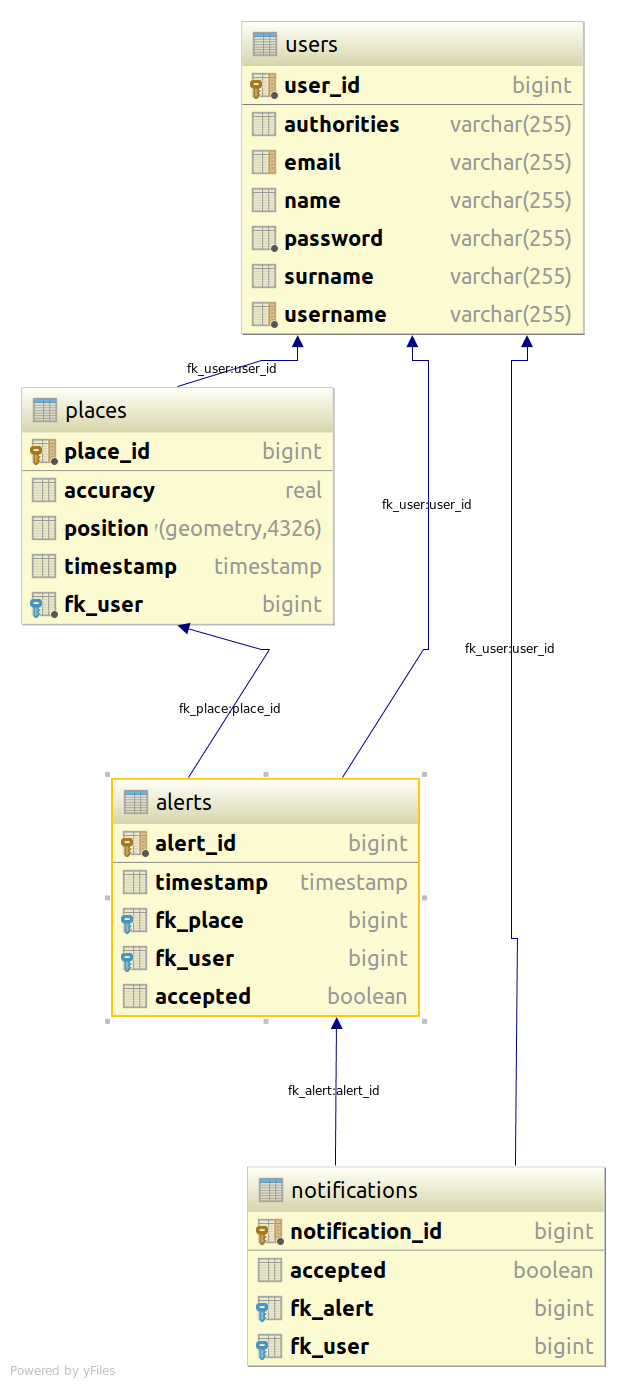
\includegraphics[width=100mm]{images/db-diagram.png}
  \caption{Μοντέλο δεδομένων}
  \label{fig:db-diagram}
\end{figure}

\clearpage

\subsection{Σύνθετα ερωτήματα}
Τέλος ένα σημείο το οποίο θα πρέπει να παραμείνουμε είναι ο τρόπος ανάκτησης δεδομένων από την επέκταση PostGIS. Παρακάτω στον αλγόριθμο ~\ref{lst:sql-query} βλέπουμε το ερώτημα το οποίο μας επιστρέφει τους χρήστες οι οποίοι βρέθηκαν στο ίδιο σημείο με κάποιο χρήστη ο οποίος έστειλε ένα συναγερμό, σε μία διάμετρο δέκα μέτρων καθώς επίσης και σε ένα συγκεκριμένο χρονικό διάστημα. 
\par
Το ερώτημα φαίνεται ιδιαίτερα απλό παρόλα αυτά χωρίς τη χρήση της επέκτασης PostGIS θα ήταν αδύνατο χωρίς τη δημιουργία πολυσύνθετων μεθόδων στη βάση δεδομένων ή στον εξυπηρετητή.

 \begin{lstlisting}[language=SQL, caption=Σύνθετο ερώτημα τοποθεσιών, label={lst:sql-query}]

select * from places p, users u where st_point_inside_circle(p.position,:longitude,:latitude,10) and p.timestamp between to_timestamp(:fromTime, 'YYYY/MM/DD hh24:mi:ss') and to_timestamp(:fromTime, 'YYYY/MM/DD hh24:mi:ss') + interval '10 minutes' and p.fk_user != :userId and p.fk_user = u.user_id;
            
\end{lstlisting}